%%%%%%%%%%%%%%%%%%%%%%%%%%%%%%%%%%%%%%%%%%%%%%%%%%%%%%%%%%%%%%%%%%%%%%%%%%%%%%%%
%%%%%%%%%%%%%%%%%%   Vorlage für eine Abschlussarbeit   %%%%%%%%%%%%%%%%%%%%%%%%
%%%%%%%%%%%%%%%%%%%%%%%%%%%%%%%%%%%%%%%%%%%%%%%%%%%%%%%%%%%%%%%%%%%%%%%%%%%%%%%%

% Erstellt von Maximilian Nöthe, <maximilian.noethe@tu-dortmund.de>
% ausgelegt für lualatex und Biblatex mit biber

% Kompilieren mit 
% latexmk --lualatex --output-directory=build thesis.tex
% oder einfach mit:
% make

\documentclass[
  tucolor,       % remove for less green,
  BCOR=12mm,     % 12mm binding corrections, adjust to fit your binding
  parskip=half,  % new paragraphs start with half line vertical space
  open=any,      % chapters start on both odd and even pages
  cleardoublepage=plain,  % no header/footer on blank pages
]{tudothesis}


% Warning, if another latex run is needed
\usepackage[aux]{rerunfilecheck}

% just list chapters and sections in the toc, not subsections or smaller
\setcounter{tocdepth}{1}

%------------------------------------------------------------------------------
%------------------------------ Fonts, Unicode, Language ----------------------
%------------------------------------------------------------------------------
\usepackage{fontspec}
\defaultfontfeatures{Ligatures=TeX}  % -- becomes en-dash etc.

% german language
\usepackage{polyglossia}
\setdefaultlanguage{english}

% for english abstract and english titles in the toc
\setotherlanguages{english}

% intelligent quotation marks, language and nesting sensitive
\usepackage[autostyle]{csquotes}

% microtypographical features, makes the text look nicer on the small scale
\usepackage{microtype}

%------------------------------------------------------------------------------
%------------------------ Math Packages and settings --------------------------
%------------------------------------------------------------------------------

\usepackage{amsmath}
\usepackage{amssymb}
\usepackage{mathtools}

% Enable Unicode-Math and follow the ISO-Standards for typesetting math
\usepackage[
  math-style=ISO,
  bold-style=ISO,
  sans-style=italic,
  nabla=upright,
  partial=upright,
]{unicode-math}
\setmathfont{Latin Modern Math}

% nice, small fracs for the text with \sfrac{}{}
\usepackage{xfrac}  


%------------------------------------------------------------------------------
%---------------------------- Numbers and Units -------------------------------
%------------------------------------------------------------------------------

\usepackage[
  locale=DE,
  separate-uncertainty=true,
  per-mode=symbol-or-fraction,
]{siunitx}
\sisetup{math-micro=\text{µ},text-micro=µ}

%------------------------------------------------------------------------------
%-------------------------------- tables  -------------------------------------
%------------------------------------------------------------------------------

\usepackage{booktabs}       % \toprule, \midrule, \bottomrule, etc

%------------------------------------------------------------------------------
%-------------------------------- graphics -------------------------------------
%------------------------------------------------------------------------------

\usepackage{graphicx}
% currently broken
% \usepackage{grffile}

% allow figures to be placed in the running text by default:
\usepackage{scrhack}
\usepackage{float}
\floatplacement{figure}{htbp}
\floatplacement{table}{htbp}

% keep figures and tables in the section
\usepackage[section, below]{placeins}


%------------------------------------------------------------------------------
%---------------------- customize list environments ---------------------------
%------------------------------------------------------------------------------

\usepackage{enumitem}

%------------------------------------------------------------------------------
%------------------------------ Bibliographie ---------------------------------
%------------------------------------------------------------------------------
\usepackage{bibstyle}
\usepackage[
  backend=biber,   % use modern biber backend
  autolang=hyphen, % load hyphenation rules for if language of bibentry is not
                   % german, has to be loaded with \setotherlanguages
                   % in the references.bib use langid={en} for english sources
]{biblatex}

\addbibresource{references.bib}  % the bib file to use
\DefineBibliographyStrings{german}{andothers = {{et\,al\adddot}}}  % replace u.a. with et al.


% Last packages, do not change order or insert new packages after these ones
\usepackage[pdfusetitle, unicode, linkbordercolor=tugreen]{hyperref}
\usepackage{bookmark}
\usepackage[shortcuts]{extdash}

%------------------------------------------------------------------------------
%-------------------------    Angaben zur Arbeit   ----------------------------
%------------------------------------------------------------------------------

\author{Cihad Gözsüz}
\title{Neural network based signal-background classification for the differnetial single top+photon measurement at the ATLAS experiment}
\date{2021}
\birthplace{Dortmund}
\chair{Lehrstuhl für Experimentelle Physik IV}
\division{Fakultät Physik}
\thesisclass{Bachelor of Science}
\submissiondate{13. July 2021}
\firstcorrector{Prof.~Dr.~Johannes Erdmann}
\secondcorrector{Prof.~Dr.~Johannes Albrecht}

% tu logo on top of the titlepage
\titlehead{
\includegraphics[height=1.5cm]{logos/tu-logo.pdf}}

\begin{document}
\frontmatter
\thispagestyle{empty}
\setcounter{page}{2}
\section*{Hinweise}
Empfohlen wird die Verwendung dieser Vorlage mit der jeweils aktuellsten TeXLive Version (Linux, Windows) bzw. MacTeX Version (MacOS).
Aktuell ist dies TeXLive 2016. Download hier:
\begin{center}
  \ttfamily\url{https://www.tug.org/texlive/}
\end{center}
Bei Verwendung von TexLive Versionen 2014 und älter sollte
die Zeile
\begin{center}
\verb+\RequirePackage{fixltx2e}+ 
\end{center}
als erste Zeile der Präambel noch vor der Dokumentenklasse eingefügt werden.
Dies lädt diverse Bugfixes für LaTeX, die ab TexLive 2015 Standard sind.

Die Vorlage \texttt{thesis.tex} ist für die Kompilierung mit \texttt{lualatex} ausgelegt, mit wenigen Anpassungen kann sie aber auch mit \texttt{pdflatex} oder \texttt{xelatex} verwendet werden. 
Die Dokumentenklasse \texttt{tudothesis.cls} kann mit allen drei Programmen verwednet werden.

Achten Sie auch auf die Kodierung der Quelldateien.
Bei Verwendung von Xe\LaTeX\ oder Lua\LaTeX\ (empfohlen) müssen die
Quelldateien UTF-8 kodiert sein.
Bei Verwendung von pdf\LaTeX\ nutzen Sie die Pakete \texttt{inputenc} und \texttt{fontenc} mit der korrekten Wahl der Kodierungen.

Eine aktuelle Version dieser Vorlage steht unter 
\begin{center}
  \ttfamily\url{https://github.com/maxnoe/tudothesis}
\end{center}
zur Verfügung.

Alle verwendeten Pakete werden im \LaTeX{} Kurs von Pep et al.\ erklärt:
\begin{center}
  \ttfamily\url{http://toolbox.pep-dortmund.org/notes}
\end{center}

Für Rückmeldungen und bei Problemen mit der Klasse oder Vorlage, bitte ein \emph{Issue} auf GitHub aufmachen oder eine Email an
\href{mailto:maximilian.noethe@tu-dortmund.de}{maximilian.noethe@tu-dortmund.de} schreiben.

Wenn Sie die Dokumentenklasse mit der Option \texttt{tucolor} laden, werden verschiedene Elemente in TU-Grün gesetzt.

\maketitle

% Gutachterseite
\makecorrectorpage

% hier beginnt der Vorspann, nummeriert in römischen Zahlen
\thispagestyle{plain}
\nocite{PhysRevLett.121.221802}

\section*{Abstract}
\begin{english}
Differential measurement of the $tq\gamma$ process in the Standard Model would enable investigations of the electromagnetic coupling of the top quark. 
Regarding this measurement of $tq\gamma$ with the full Run-2 dataset at the ATLAS experiment, a neural network is trained on data from Monte Carlo simulations to discriminate background processes from the $tq\gamma$ signal process. 
Certain features of events are provided as input to the neural network. 
In this thesis, the influence of these input features on the neural network's ability to separate signals from the background is investigated. This provides insights into which event features are essential characteristics to understand the electromagnetic coupling of the top quark.
\end{english}

\tableofcontents

\mainmatter
% Hier beginnt der Inhalt mit Seite 1 in arabischen Ziffern

\chapter{Introduction}


The standard model of particle physics (SM) describes the nature of discovered elementary particles and three of the four fundamental interactions: strong, weak and electromagnetic interaction. 
All observed microscopic phenomena can be attributed to one of these interactions. Only the gravitational interaction is not covered by the theory.  Therefore, the SM is widely regarded as the most successful theory and has been researched extensively. 
However, there remain several problems of the SM. For instance, the theory cannot explain the origin of its fundamental parameters. Furthermore, the existence of dark matter is also not accounted for in the SM. The many problems of the SM motivate the search for physics beyond the Standard Model (BSM). 
It is therefore essential to test and research the limits of this theory.\\
 Many tests of the Standard Model involve the top quark, the most massive elementary particle. One such test would be the search for the production of a single top in association with a photon in proton-proton-collisions ($pp \rightarrow tq\gamma$). 
The process is sensitive to the top quark coupling to the $W$ boson and the photon. As these couplings are one of the critical parameters of the SM, a precise measurement of the cross-section for this process may give new insights into these parameters. \\
 A large number of background processes occupy the measurement region of $tq\gamma$. Major background processes are $t\bar{t}\gamma$, $W\gamma$ and $t\bar{t}$ with smaller contributions from other processes. A classifying neural network is implemented to differentiate 
the signal process $tq\gamma$ from the background processes. This neural network is trained on simulated data and receives kinematic and topological event variables as the input. 
When training a neural network, the influence of the input parameters on the output of the neural network is unknown. However, studying the significance and effects of different input parameters on the output would provide key insights for optimising of the neural network. 
Additionally, this study may help narrow down or provide new conditions for the event selection criteria to optimise background noise suppression. Finally, the investigation of these input features could provide vital insights into the nature of the $tq\gamma$ process. 
In this thesis, the correlations of input features and additional event parameters with the neural network output are calculated and analysed. Subsequently, two input features, the transverse momentum of the photon $p_T^\gamma$ and the energy of the forward jets with the photon energy, are chosen to be further studied. 
These features are cut to specific energy regions. The effects of different cuts on the neural network are then thoroughly examined and discussed. 



\chapter{Single top quark production with a photon in the Standard Model}
\label{chap:tqgamma_production}
\section{A brief overview of the Standard Model}

The Standard Model (SM) of particle physics, a quantum field theory,  describes today's best theory of particle physics. 
In the SM, there are different kinds of elementary particles and three fundamental forces of nature: the electromagnetic force, the strong force and the weak force. 
Every force coincides with an elementary particle, called a boson, that acts as a mediator of the interaction. Another group of particles are called the fermions, and they only interact with these bosons if they have specific quantities, which are represented by their quantum numbers.

The fermions have spin $s = \frac{1}{2}$ and can be divided into two separate groups. The first group, named quarks, are colour charge carrying fermions. 
There are three up-type quarks (up, strange and top) with an electric charge of $q = +\frac{2}{3}e$ and three down-type quarks (down, charm and bottom) with an electric charge of $q = -\frac{1}{3}e$. 
The second group are the leptons. Three leptons (electron, muon and tau) have an electric charge of $q = +1e$. Furthermore, each of these leptons has a corresponding uncharged lepton partner called a neutrino.
Three different families further categorize leptons and quarks. These quark and lepton families are ordered by mass and consist of an up-type quark, the corresponding down-type quark, a lepton and the corresponding neutrino. 
There is an anti-matter particle equivalent for all fermions where every charge-like quantum number has the opposite sign. 

Particles with integer spin are called bosons. The first group of bosons, gauge bosons with spin $s = 1$, mediate the three fundamental forces. The gauge bosons with spin $s = 1$ are: $gluons$ $g$, $photons$ $\gamma$, $Z$ and $W^{\pm}$. The Higgs boson $H$ is the only boson with spin $s=0$.

Gluons are colour charged and mediate the strong force between colour charged particles, including themselves. The six colour charges are $red$,$green$,$blue$ and their anticolour counterpart. The strong force draws particles with colour together until a colour neutral state is achieved. This can occur when one quark bonds with a quark of the opposite colour, forming a meson. It can also occur when three quarks with $red$, $green$, $blue$ colour charges respectively together form the colour neutral Baryon. 
The strong force becomes stronger the further quarks are repelled from the colour neutral state. If quarks get repelled for a sufficiently high distance, two new quarks are formed, which then bond with the repelled. This process is called colour confinement and can occur many times in a row for higher energies, forming a shower of mesons and baryons. 
Photons mediate the electromagnetic (EM) between electrically charged particles. The massive bosons, $Z$ and $W^{-}$ as well as $W^{+}$ mediate the weak force. The weak force only acts on left-handed particles (and right-handed antiparticles). Here, left-handedness means that the spin direction is opposite to the direction of the momentum of the particle. Right-handed particles have their spin and momentum pointing at the same direction. 
The $W^{\pm}$ bosons are electrically charged, $q = \pm 1e$, and change the flavour of a quark when coupling to it. The flavour refers to the species of a fermion. 
 
The Higgs boson arises from the electroweak theory. The Higgs mechanism provides an explanation for the presence of massive leptons and bosons by breaking the electroweak symmetry. The fermions acquire their mass by coupling with the Higgs boson via the so-called Yukawa interaction.
Before the breaking of the electroweak symmetry, the gauge bosons exist as the electroweak eigenstates $W^1$, $W^2$, $W^3$ and $B$. The breaking of this symmetry mixes $W^3$ and $B$ into the mass eigenstates $Z$ and $\gamma$. 
The eigenstates $W^1$ and $W^2$ mix into the massive eigenstates $W^+$ and $W^-$. 

An overview of the elementary particles in the Standard Model is given in figure \ref{fig:standard_model}.

\begin{figure}
    \centering
    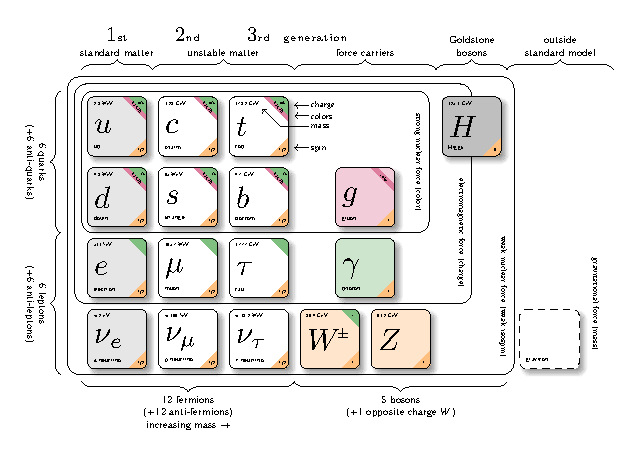
\includegraphics[width=0.6\textwidth]{Plots/model-physics.pdf}
    \caption{Elementary particles of the Standard Model alongside their properties \cite{sm_table}.}
    \label{fig:standard_model}
\end{figure}

\section{The \texorpdfstring{$tq\gamma$}{tqGamma} process in the Standard Model}
\label{sec:tqgammainsm}

The top quark is an up-type quark and the most massive quark of the Standard Model with a mass of $m_t = 173.76 \pm 0.3 \,\si{\giga\electronvolt} (S =1.2)$ \cite{pdg}. Additionally, the top quark has a very small decay width of $\Gamma = 1.42^{+0.19}_{-0.15} \,\si{\giga\electronvolt} (S=1.4)$ \cite{pdg} because of its high mass.
This is one reason why the top quarks unlikely to build any bound states and always decay shortly after production. Only their decay products are observable and can be retraced back to the top quark. 

Top quarks can be produced in three different channels: In the $t$-channel ($tq$), where a single top quark is produced when a bottom quark exchanges a $W$-boson with another quark, the $s$-channel ($tb$), where the top quarks are produced in top-antitop-pairs, and the $tW$-channel, where a gluon and a bottom couple and then decay into a single top and a $W$ boson. In this thesis, the focus lies primarily on the $t$-channel production of the top quark. 
The top quark was first discovered in pair production at the Tevatron in 1995 during a proton-antiproton collision experiment (CITE). In 2009, the D0 \cite{singletop1} and CDF \cite{singletop2} collaborations also separately confirmed the observation of the $t$-channel top quark production at the Tevatron. The combined results are available in reference \cite{singletop3}. 
The CMS experiment at the Large Hadron Collider (LHC) of CERN \cite{CMS} reported evidence for the $t$-channel single production of top quarks in association with a photon ($tq\gamma$) with a significance corresponding to $\sigma = 4.4$. The fiducial cross section 
was measured to be $\sigma(pp\rightarrow tq\gamma)(t\rightarrow\mu \nu b) = 115 \pm 17 (stat) \pm 30 (syst) \,\si{\femto\barn}$ for the photon transverse momentum $p_T^\gamma > 25 \,\si{\giga\electronvolt}$ \cite{PhysRevLett.121.221802}. 

For this thesis, the $tq\gamma$-events are produced in proton-proton-collisoins inside the ATLAS experiment. The ATLAS is discussed in detail in chapter \ref{chap:measurement}. The production of processes in this experiment occurs with elementary particles inside of the protons, called partons. For the production of the $tq\gamma$-process, one gluon provided by the protons may produce a bottom-antibottom-quark pair. The bottom quark may then exchange a $W$-boson with a quark, turning the bottom quark into a top quark and changing the flavour of the quark. This top quark may then radiate a photon. 
It is essential to mention that while this thesis focuses on the top-photon vertex, the photon can be radiated from any charged particle elsewhere in the process. For instance, the bottom quark after the decay of the top may produce a photon.
Afterwards, the top quark decays decays into a $W^+$-boson and a bottom quark. The $W^+$-boson then decays either into an antilepton and neutrino pair or a quark-antiquark pair of opposite quark types. However, only the leptonic decay mode is considered in this thesis.

In Figure \ref{fig:feyn_tqGamma} the leading order Feynman diagram for the $tq\gamma$ production is depicted. The charge conjugated diagram is not shown, but also considered in this thesis.
\begin{figure}
    \centering
    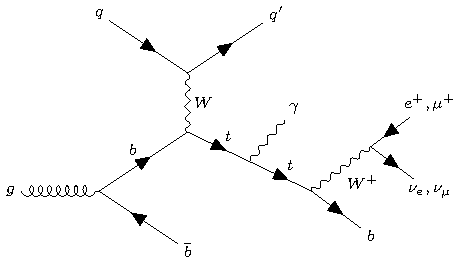
\includegraphics[width=0.6\textwidth]{Plots/s4_feyn_nom.pdf}
    \caption{Leading order Feynman diagram of the $tq\gamma$ process in the Standard Model.}
    \label{fig:feyn_tqGamma}
\end{figure}



\chapter{Measurement of \texorpdfstring{$tq\gamma$}{tqGamma}}
\label{chap:measurement}

\begin{enumerate}
    \item Explain why $t\bar{t}\gamma$ is close to $tq\gamma$. Mit crossection
    \item Anit $k_t$ besser erklären
    \item Reconstruction of leptons
    \item Reconstruction of photons
\end{enumerate}
\section{The ATLAS Experiment}
\label{sec:atlas}
The European Organization for Nuclear Research, known as CERN, located in Geneva, has various experiments studying elementary particles through the collision of heavy ions and protons. 
The Large Hadron Collider (LHC), the largest particle accelerator of CERN, has a circumference of $27 \,\si{\kilo\metre}$ and can collide particles with a center of mass energy of up to $\sqrt{s} = 13.6 \,\si{\tera\electronvolt}$. 


The LHC consists of four extensive experiments: the ALICE, the LHCb, the CMS and the ATLAS experiments. The research in this thesis is done with the help of the largest of these experiments, the ATLAS experiment. Figure 1 visualizes the structure of the ATLAS detector. 
A coordinate system needs to be defined in order to discuss the construction of the experiment. Three different coordinates are used to describe positions inside the experiment: First, the azimuthal angle $\phi$, which ranges from $0$ to $2\pi$. 
Next, the pseudorapidity $\eta$, which is defined to be $\eta = -\ln(\tan \theta)$, where $\theta$ is the angle to the beam axis. The smaller $\theta$ is, the higher the pseudorapidity. And lastly, a distance $\Delta R$, which can be defined in the $\phi$-$\theta$-plane as $\Delta R = \sqrt{(\Delta \phi)^2 +(\Delta \eta)}$.

The ATLAS detector is built symmetrically around the particle beam and can be divided into three subdetectors:

The inner detector tracks charged particles just after the collision. 
It consists of three different systems of sensors in a magnetic field parallel to the beam. 
These sensors are the pixel detector, the semiconductor tracker which works with silicone strips and a transition radiation tracker to track particles with gas-filled tubes. 

In the EM calorimeter, metal layers (tungsten, copper or lead) absorb incoming particles and convert them into lower-energy particles called a shower. The calorimeters detect "showers" produced by electrons (and positrons), photons and hadrons. The barrel part of this calorimeter covers the pseudorapidity range $|\eta| < = 1.475$ and the end-cap components cover $1.375 <|\eta|< 3.2$.
Hadrons do not deposit all of their energy into the EM calorimeter; they get absorbed by steel layers in the hadronic calorimeter. 
Plastic scintillating tiles then produce photons that get converted into an electric current. The scintillating tiles cover the region $|\eta| < 1.7$. The region $1.5 < |\eta| < 4.9$ is then used by the cooper + liquid argon and tungsten + liquid argon calorimeter.

The muon spectrometer measures trajectories of muons with the help of a magnetic field. The spectrometer detects muons in the range of $\bigl|\eta\bigr| > 2.7$. 
Monitored drift tubes measure pseudorapidities up to $|\eta| = 2.0$ and cathode strip chambers cover higher pseudorapidities.  
\begin{figure}
    \centering
    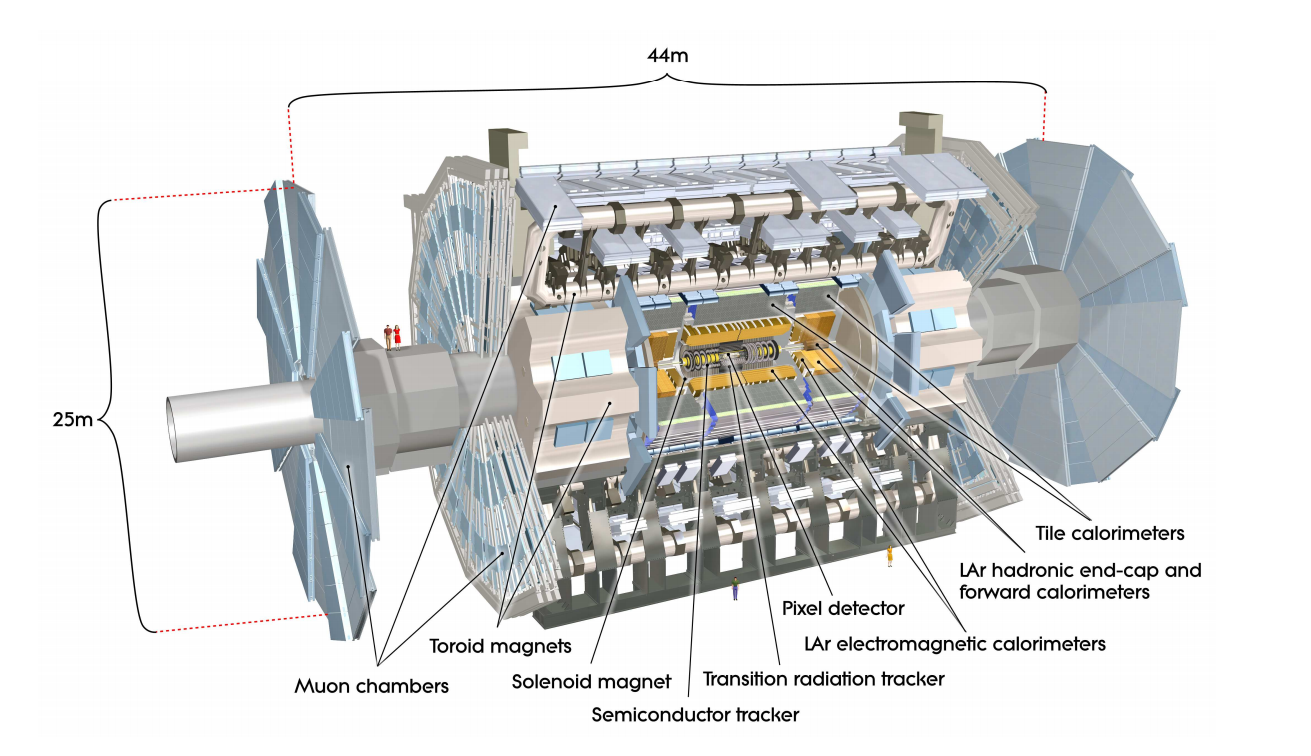
\includegraphics[width=0.9\textwidth]{Plots/atlasSCHEMA.PNG}
    \label{fig:atlasschema}
    \caption{Schematic visualisation of the ATLAS Detector \cite{Collaboration_2008}.}
\end{figure}



\section{Object Reconstruction at the ATLAS experiment}

\subsection{Reconstruction of photons}
\label{sec:reconphoton}
?
\subsection{Reconstruction of leptons}
\label{sec:reconlepton}
?
\subsection{Jets}
\label{sec:jets}
Jets are reconstructed from clusters of energy depositions of mostly mesons and fewer baryons that result from the separation of two quarks (color confinement) (\textbf{NOTE: }Jets sind tatsächlich ausschließlich Schauer aus quarks. EM-Schauer sind keine Jets). They are reconstructed with the help of the anti-$k_t$ algorithm \cite{anti_k_t} with a radius parameter of $R = 0.4$. 
This algorithm reconstructs jets by first identifying the particle source via the jet energy scale. It is then required that the jet has a transverse momentum of $p_T > 25 \,\si{\giga\electronvolt}$ and $\bigl|\eta\bigr| < 4.5$. 

Detector noise can lead to the misidentification of a jet. The nature of these misidentified jets has been studied thoroughly \cite{70} and a so-called "jet cleaning procedure" is used to tag them. 
Any event containing at least one "bad" jet is removed. 

\subsection{Missing transverse momentum \texorpdfstring{$E_T^{\text{miss}}$}{}}

If all particle products are considered, there should be no magnitude for the sum of the transverse momentum $p_T$ of all particles. 
Any measured magnitude is therefore attributed to an unmeasured particle. The missing transverse energy $E_T^{\text{miss}}$ is consequently defined as the negative of this sum and assinged to a neutrino. 

\section{Background contributions from similar processes}



Various different processes besides $tq\gamma$ are also accepted by the criteria for event selection \ref{sec:eventselect}. For the scope of this thesis, contributions from these processes are considered background.  
The process $t\bar{t}\gamma$ holds the most similar decay product as it's products can be identical to the products of $tq\gamma$. %EXPLAIN WHY WITH CROSSSECTION
Following processes is the production of a $W$-boson with jets, a $Z$-boson with jets and $t\bar{t}$.

Table \ref{tab:background} lists these and the rest of the processes contributing to the background.
\begin{table}
    \centering
    \begin{tabular}{c c c}
        \toprule
        {} & Process \\
        \midrule
        1 & $tq\gamma$\\[.1cm]
        2 & $t\bar{t}\gamma$\\[.1cm]
        3 & $W\gamma + jets$\\[.1cm]
        4 & $Z\gamma + jets$\\[.1cm]
        5 & $t\bar{t}$\\[.1cm]
        6 & $s\-chan$\\[.1cm]
        7 & $t W$\\[.1cm]
        8 & $t\-chan$\\[.1cm]
        9 & $VV$\\[.1cm]
        10& $W+jets$\\[.1cm]
        11& $Z+jets$\\[.1cm]
        \bottomrule
    \end{tabular}
    \caption{List of SM processes that contribute to background noise in the measurement of $tq\gamma$.}
    \label{tab:background}
\end{table}






\chapter{Monte Carlo samples and event selection}


\section{Generation of Monte Carlo samples}
\label{sec:mc}
The framework \textsc{MadGraph5\_aMC@NLO} is used for Monte Carlo (MC) simulations of the considered $tq\gamma$ process. \textsc{MadGraph5} is a matrix element generator that allows the interfacing of different packages for further simulation. 
The simulated events are generated at next-to-leading order (NLO) at the $t$-channel of single top production. The generator is interfaced to the package \textsc{Pythia} $v8.240$, which provides parton showers. 
The \textsc{MadSpin} and \textsc{EvtGEN} $v1.6.0$ packages give decay simulations of the top and bottom quark, respectively. Here, only leptonic decays of the top quark are considered.

Moving on to background processes, the $t\bar{t}$ process is modelled at leading order (LO) also using \textsc{MadGraph5\_aMC@NLO} $v2.3.3$ interfaced to \textsc{Pythia} $v8.212$. 
Simulation of $W\gamma$+jets and $Z\gamma$+jets events are produced at NLO using the \textsc{Shepra} $v2.2.2$ and \textsc{Shepra} $v2.2.4$ packages. For the $t\bar{t}$ process and $t$-, $s$-, $tW$-channels 
\textsc{Powheg-Box} is used where \textsc{Pythia} $v8.230$ is again used as the showering program. The modeling here is performed in NLO in QCD. 

The table \ref{tab:eventgen} gives a summary of the generated samples and their generators.

\begin{table}
    \centering
    \begin{tabular}{c|c}
        \toprule
        Process & Generator\\
        \midrule
        $tq\gamma$&$MadGraph5\_aMC@NLO$ + $Pythia8$\\[.1cm]
        $t\bar{t}\gamma$&$MadGraph5$ + $Pythia8$\\[.1cm]
        $W\gamma + jets$&$Sherpa$ $2.2.2$\\[.1cm]
        $Z\gamma + jets$ &$Sherpa$ $2.2.4$\\[.1cm]
        $t\bar{t}$ &$Powheg$ + $Pythia8$\\[.1cm]
        single top&$Powheg$ + $Pythia8$\\[.1cm]
        $W+jets$& $Sherpa$ $2.2.1$\\[.1cm]
        $Z+jets$ &$Sherpa$ $2.2.1$\\[.1cm]
        Diboson &$Sherpa$ $2.2.2$\\
        \bottomrule
    \end{tabular}
    \caption{List of generated samples alongside their generators.}
    \label{tab:eventgen}
\end{table}
\section{Event selection}
\label{sec:eventselect}
The selection criteria for events must hold the necessary conditions for a $tq\gamma$-process. It also needs to have enough restrictions to reduce background contributions as much as possible. 
Signal events have precisely one lepton, at least one photon and one $b$-tagged jet in the final state. The lepton should have a transverse momentum higher than $20 \,\si{\giga\electronvolt}$, the photons momentum higher than $27\,\si{\giga\electronvolt}$ and 
the $b$-tagged jet has to pass the $DL1r$-algorithm with a $70\%$ working point.\\
Additionally, the missing transverse energy $E_T^{miss}$ ought to be above $30 \,\si{\giga\electronvolt}$ to account for the neutrino in the decay mode. 
Finally, to reduce leading background contributions from the $Z \rightarrow ee(\rightarrow \gamma)$ process, the invariant mass of the leading photon and an electron candidate $m_{e\gamma}$ is set to be in the range $80 \,\si{\giga\electronvolt} < m_{e\gamma} < 110 \,\si{\giga\electronvolt}$.
Altogether, this makes up the following requirements for selected events:
\begin{enumerate}
    \item At least one photon $\gamma$ with $p_T > 20 \,\si{\giga\electronvolt}$
    \item Exactly one lepton with $p_T >27\,\si{\giga\electronvolt}$
    \item $E_T^{miss} > 30 \,\si{\giga\electronvolt}$
    \item Exactly one $b$-tagged jet passing $70\%$ working point (WP) of the $DL1r$-algorithm. 
    \item Invariant mass of leading photon and electron candidate between values $80 \,\si{\giga\electronvolt} < m_{e\gamma} < 110 \,\si{\giga\electronvolt}$  
\end{enumerate}
\chapter{The Neural Network used for signal-background classification}
\section{Short introduction to neural networks}
Neural networks are loosely on the human brain and are a means of doing machine learning, in which a computer learns to perform some task by analyzing training examples. 
A NN is usually organized into layers of processing nodes. These processing nodes are densely interconnected between layers, and every connection weighted. 
During the $forward$ $propagation$, where the NN is tested on provided data, computations in the NN propagate from the input layer to the output layer. An individual node receives data from nodes in the layer beneath it and sends data to nodes in the layer above. 
Nodes multiply received data by their weight value and add them together to a single value. Only if the node exceeds a specific threshhold does it send its value to the next layer. During $backpropagation$, where the NN is being trained, weights and thresholds are continually adjusted until training data with the same label yield similar results.   
In this thesis, a NN discriminates between the $tq\gamma$ signal and background events. 
The NN is trained on Monte Carlo simulations (Section \ref{sec:mc}) and is tested on measurement data after that. Characteristic variables of events, which are discussed in detail in section \ref{sec:inputfeatures}, are used as the input. 
\section{The neural network architecture}
\label{sec:arch}
The NN are built using the \texttt{Keras} library running on \texttt{TensorFlow} \cite{Keras} \cite{tensorflow}.
Two different neural networks are trained to separate the signal from the background. One is trained on the zero-forward jet signal region ($0\text{-}fj$), and the other is trained on the At least one forward jet region ($\geq 1\text{-}fj$). 
This is done to optimize the sensitivity of the analysis as the signal to background ratio ($S/B$) is greater for the $\geq 1\text{-}fj$ region than the $0\text{-}fj$ region. \\
Both models consist of one input layer, three densely connected node layers (Dense layer) and one output layer. The input layers have nodes for each input feature. The NN for $0\text{-}fj$ events has $16$ input features while the NN for $\geq 1\text{-}fj$ events has $27$ due to additional variables of the forward jets. 
The activation function for the Dense layers is the Leaky Rectified Linear Unit (ReLU) function $f(x)$:
\begin{align*}
    f(x) =\begin{cases}
            x, & \text{for } x \geq 0\\
            0.5x, & \text{for } x < 0.
        \end{cases}
\end{align*}
For the output layer, the activation function is the sigmoid function $\sigma(x)$:
\begin{align*}
    \sigma(x) = \frac{1}{1+ e^{-x}}. 
\end{align*}
Finally, the \texttt{Adam} algorithm is used as the optimizer for updating the weights in the NN \cite{Adam}. Figure \ref{fig:models} displays the described architecture of the NN models. 
\begin{figure}
    \centering
    \begin{subfigure}{.5\textwidth}
      \centering
      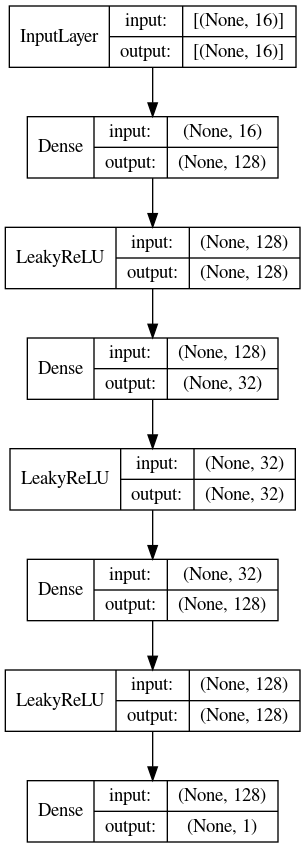
\includegraphics[width=.4\linewidth]{Plots/model_0fj.png}
    \end{subfigure}%
    \begin{subfigure}{.5\textwidth}
      \centering
      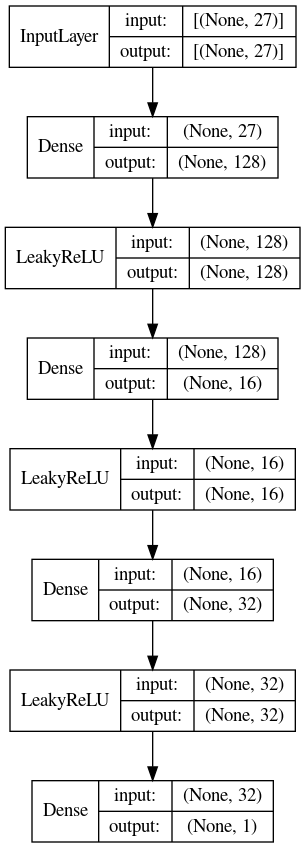
\includegraphics[width=.4\linewidth]{Plots/model_1fj.png}
    \end{subfigure}
    \caption{Visualization of the NN architecture for the zero forward jet region (left) and the $\geq 1$ forward jets region (right).}
    \label{fig:models}
\end{figure}

\section{Input features for the neural network}
\label{sec:inputfeatures}
\begin{table}
    \centering
    \begin{tabular}{c|c|c}
        \toprule
        {} &                     0fj variables      & 1fj variables\\
        \midrule 
        1  &                                HT      & HT\\ \hline
        2  &                           blep\_dr     & blep\_dr\\ \hline
        3  &                           lbj\_eta     &lbj\_eta\\ \hline
        4  &                            lbj\_pt     &lbj\_pt\\ \hline
        5  &  lbj\_tagWeightBin\_DL1r\_Continuous   & lbj\_tagWeightBin\_DL1r\_Continuous\\ \hline
        6  &                          lep1\_eta     & lep1\_eta\\ \hline
        7  &                           met\_met     &met\_met\\ \hline
        8 &                             ph\_pt     &ph\_pt\\ \hline
        9 &                             top\_m     & top\_m\\ \hline
        10 &                       transMassWb      &transMassWb\\ \hline
        11  &                            bph\_pt     & bph\_m\\ \hline
        12 &                          topph\_pt     &topph\_ctheta\\ \hline
        13 &                            ph\_eta     & ph\_phi\\ \hline
        14 &                          lepph\_dr     & lep1\_pt\\ \hline
        15 &                      transMassWph      & met\_phi\\ \hline
        16 &                           lep1\_id     & lbj\_phi\\ \hline
        17 &&                                           Wbsn\_e \\ \hline
        18 &&                                            bfj\_m \\ \hline
        19 &&                                           blep\_m \\ \hline
        20 &&                                           fj\_eta \\ \hline
        21 &&                                           fj\_phi \\ \hline
        22 &&                                        fjet\_flag \\ \hline
        23 &&                                      fjph\_ctheta \\ \hline
        24 &&                                        fjph\_deta \\ \hline
        25 &&                                          fjph\_dr \\ \hline
        26 &&                                           fjph\_e \\ \hline
        27 &&                                           fjph\_m \\ \hline
        \bottomrule 
    \end{tabular}
    \caption{Input variables of the NN trained on events with no forward jets and the NN trained on events with at least one forward jet.}
    \label{tab:features}
\end{table}


\section{Performance and distribution of the NN output}

\begin{figure}
    \centering
    \begin{subfigure}{.5\textwidth}
      \centering
      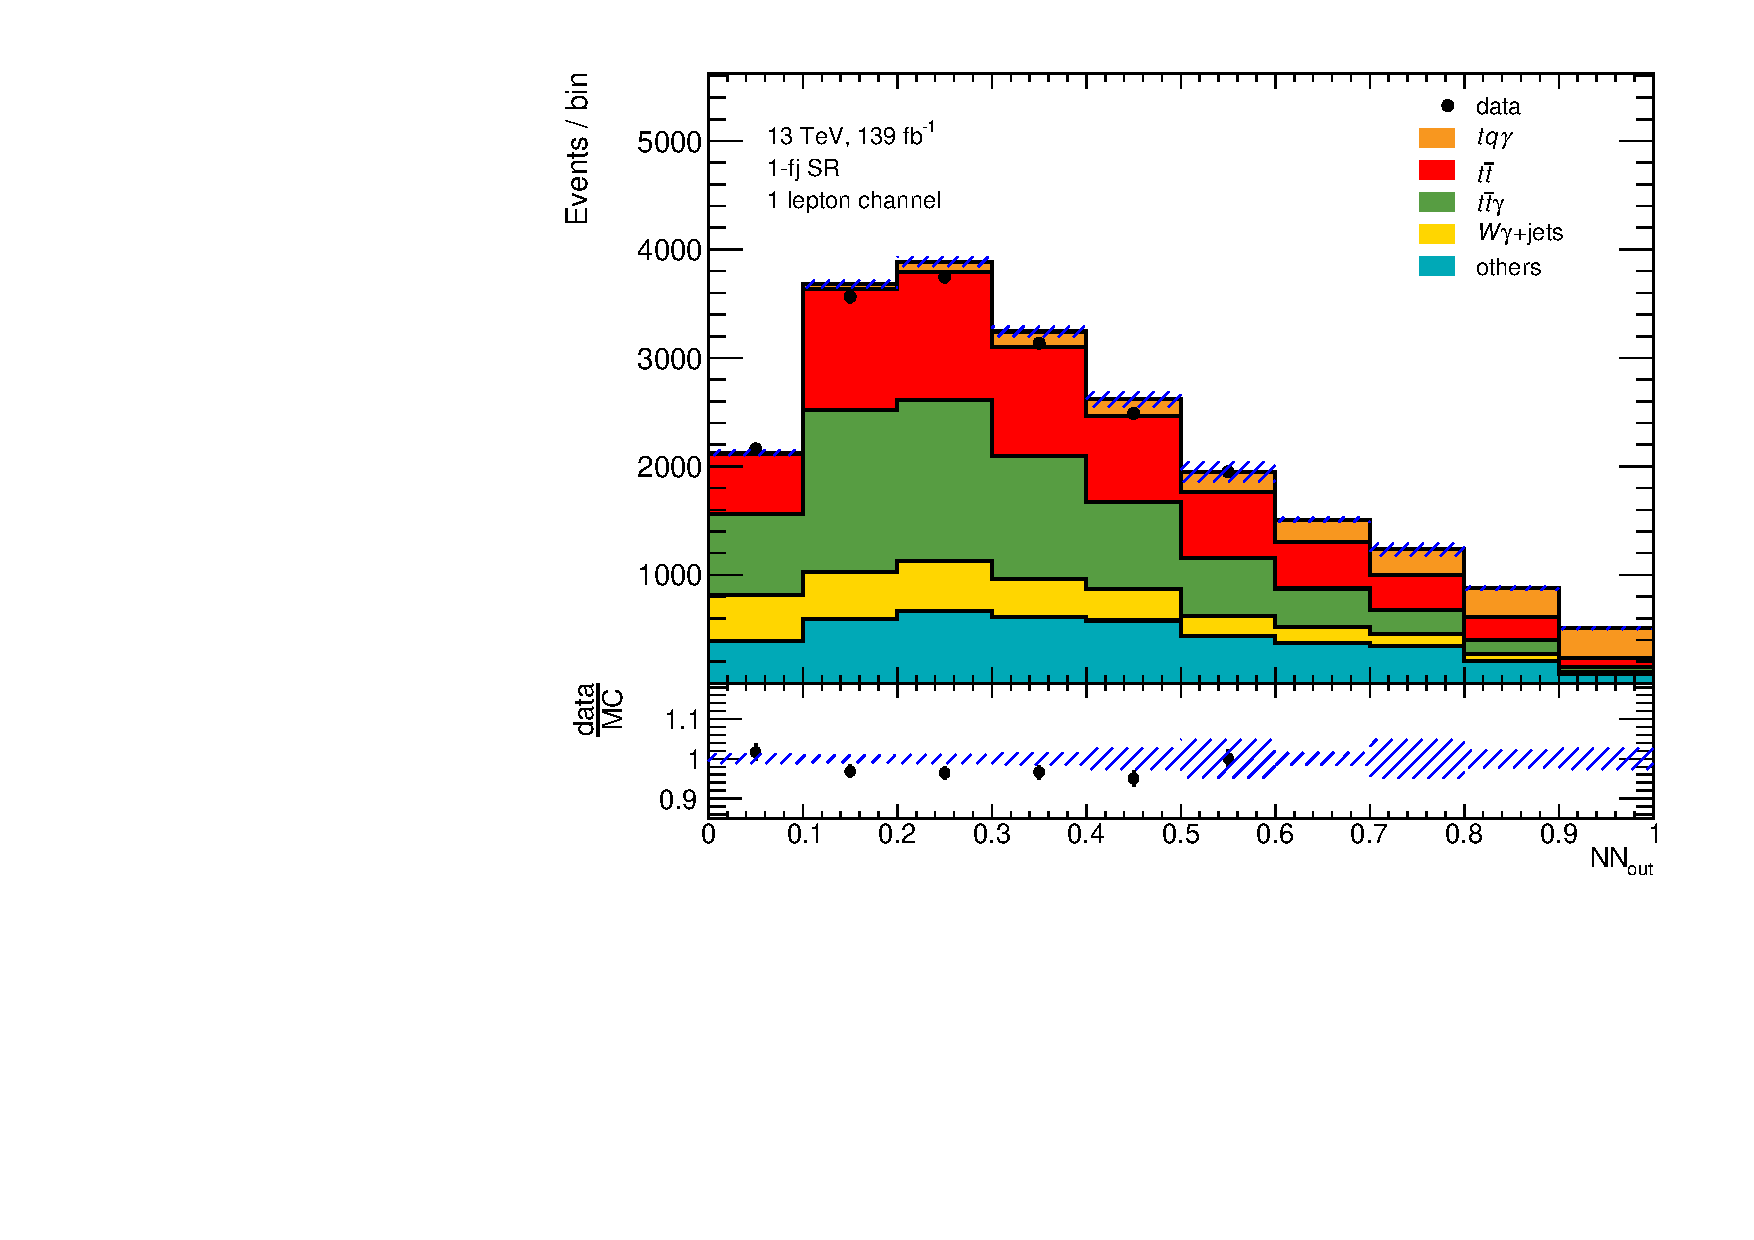
\includegraphics[width=\linewidth]{Plots/NN_out_mix_GANZ.pdf}
    \end{subfigure}%
    \begin{subfigure}{.5\textwidth}
      \centering
      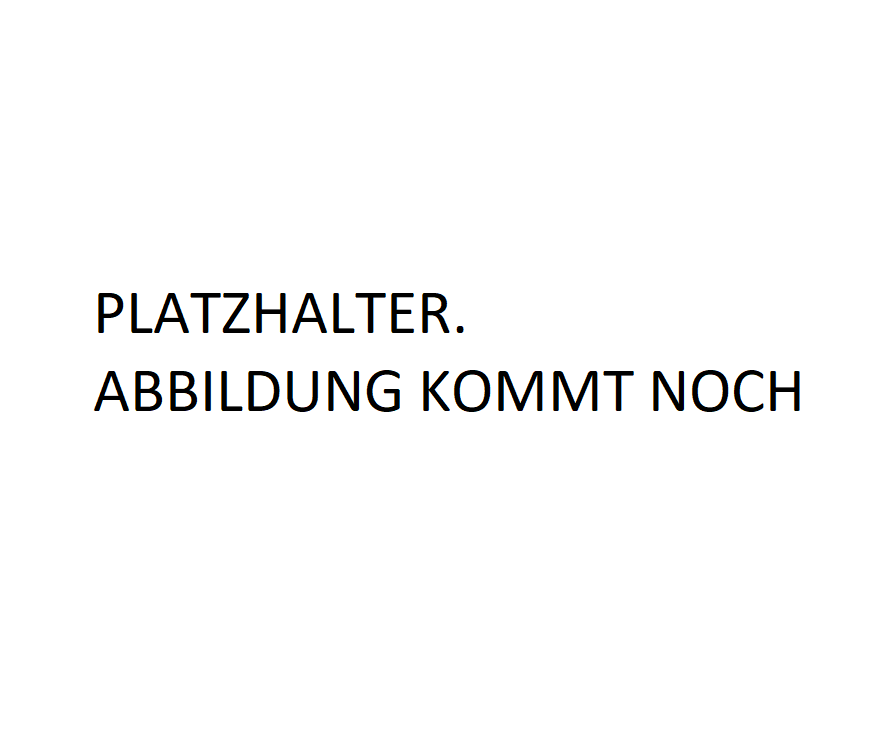
\includegraphics[width=\linewidth]{Plots/Platzhalter.png}
    \end{subfigure}
    \caption{The NN output event distribution (left) and the composition of different bins of the NN output (right).}
    \label{fig:NNdistro}
\end{figure}
\begin{figure}
    \centering
    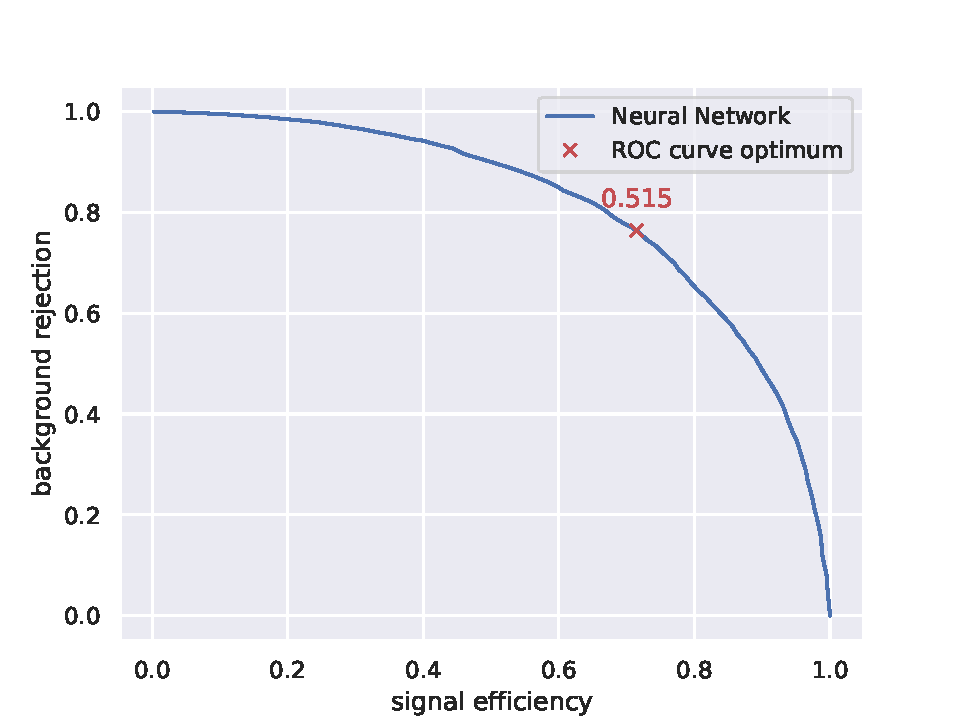
\includegraphics[width=0.5\textwidth]{Plots/ROC-Curve-fullt.pdf}
    \caption{ROC curve of the neural network with the point of maximumized signal efficiency and backgrund rejection.}
    \label{fig:rocfull}
\end{figure}
\chapter{Differnetial analysis of the NN output}
%\chapter{Analysis of the effects of different event features on the neural network output}
\section{Weighted correlations of input features with the NN output}

\subsection{Motivation for calculating correlations}
Correlations between input variables and the neural network's provide an overview of what the NN has "learned". 
They represent which input variables have the strongest influence on the output of the NN. 
The level of influence of any input variable is determined during the training phase of the NN. For example, suppose the value of a specific input variable turns out to be an essential parameter in the discrimination of the signal from the background. 
In that case, this variable will acquire a high correlation after the training process. 
Consequently, highly correlated variables would provide a critical basis to determine which properties of the $tq\gamma$ process help in understanding the photon to top quark coupling.  \\

\subsection{Steps of calculation}

Weighted correlations between two sets of data are calculated by first determining the covariance of these sets. For the covariance, the weighted mean of each set is needed. 
The weighted mean is calculated as follows
\begin{align*}
    m(x;w) &= \frac{\sum_i{w_i x_i}}{\sum_i{ w_i}}
\end{align*}
where $x$ is the given set over which to calculate the mean. In this section, $x$ represents one input feature of a process or the NN output values. The weights of each data point is given by $w$. 
The covariance is then calcuted with the formula 
\begin{align*}
    cov(x,y;w) &= \frac{\sum_i{w_i \cdot (x_i - m(x;w)) \cdot (y_i - m(y;w))}}{\sum_i{w_i}}.
\end{align*}
Here, $y$ stands for the second data set. Finally, the weighted correlation is then determined to be 
\begin{align*}
    corr(x,y;w) &= \frac{cov(x,y;w)}{\sqrt{cov(x,x;w)\cdot cov(y,y;w)}}.
\end{align*}
Thus, the correlation between the values for one input feature $X_\text{input}$ and the NN output values $Y_\text{output}$ with the weights $W$ would be $corr(X_\text{input},Y_\text{output};W)$.

Calculations for the $0\, fj$ region and the $\geq 1\, fj$ region are done separately.  
Every generated event is saved with 110 different features, including the input features, the NN output value and the NN weights. 
At the start, the calculation for variable correlations with the NN output is performed for all events of the same sample.  
Then, all correlations of the background samples are combined. This is done by calculating a weighted mean over all samples. Here, the sum of weights in a sample is used as the new weight for the mean.
Finally, the correlation of measured data is also determined. The final result is a correlation table for the whole background, the $tq\gamma$ process and the measured data in each forward jet region. 
The result of the calculations is visualised and discussed in Section \ref{sec:corrvis}.


\subsection{Visualisations of calculated correlations}
\label{sec:corrvis}
The results of the calculations are listed in Table \ref{tab:corrAll}. This table also contains some correlations of features that are not part of the input of the NN in the given region.  
Figure \ref{fig:corr0fj} and \autoref{fig:corr1fj} display correlations of the input features in order for both forward jet regions respectively. 

\textbf{Spreche über einige variablen und erkläre warum Sie stark oder weniger stark korreliert sind. Dann muss auch ph\_pt angesprochen werden. Anschließend kann fjph\_e mit fj\_e verglichen werden.}

\begin{table}[htbp]
    \centering
    \begin{tabular}{c|c c c|c c c}
        \toprule
        {}&\multicolumn{3}{c}{$0\, fj$ region}&\multicolumn{3}{c}{$\geq 1\, fj$ region}\\
        Event parameter &  Background &  $tq\gamma$ &  Data &  Background &  $tq\gamma$ &  Data \\
        \midrule
        top\_m                            & -0.51 &      0.01 &   0.03 & -0.41 &      0.06 &   0.04 \\ \hline
        Wbsn\_e                           & -0.35 &     -0.02 &   0.00 & -0.38 &      0.00 &  -0.00 \\ \hline
        blep\_m                           & -0.39 &      0.01 &   0.01 & -0.33 &      0.02 &   0.01 \\ \hline
        topph\_ctheta                     & -0.28 &     -0.00 &     & -0.33 &     -0.01 &   0.02 \\ \hline
        transMassWb                      & -0.47 &     -0.00 &     & -0.33 &     -0.02 &  -0.02 \\ \hline
        lep1\_pt                          & -0.36 &        &     & -0.32 &      0.54 &   0.43 \\ \hline
        HT                               & -0.21 &     -0.24 &  -0.35 & -0.30 &     -0.22 &  -0.32 \\ \hline
        met\_met                          & -0.26 &     -0.05 &   0.02 & -0.26 &      0.00 &  -0.01 \\ \hline
        topph\_pt                         & -0.02 &     -0.12 &  -0.14 & -0.18 &     -0.06 &  -0.03 \\ \hline
        blep\_dr                          & -0.15 &     -0.06 &  -0.14 & -0.14 &     -0.05 &  -0.07 \\ \hline
        bph\_pt                           & -0.08 &     -0.03 &   0.02 & -0.13 &      0.00 &   0.02 \\ \hline
        transMassWph                     & -0.17 &      0.00 &  -0.00 & -0.10 &      0.00 &   0.02 \\ \hline
        fjph\_dr                          &  0.00 &      0.18 &   0.19 & -0.06 &      0.14 &   0.15 \\ \hline
        lbj\_pt                           & -0.12 &     -0.32 &  -0.50 & -0.05 &     -0.24 &  -0.42 \\ \hline
        fjph\_deta                        &  0.00 &     -0.36 &  -0.29 & -0.03 &     -0.29 &  -0.33 \\ \hline
        fj\_phi                           & -0.00 &     -0.09 &  -0.08 & -0.03 &     -0.11 &  -0.19 \\ \hline
        lep1\_eta                         &  0.02 &     -0.30 &  -0.37 & -0.02 &     -0.28 &  -0.39 \\ \hline
        met\_phi                          &  0.00 &      0.27 &   0.14 & -0.01 &      0.25 &   0.18 \\ \hline
        lep1\_id                          & -0.16 &     -0.27 &  -0.43 & -0.00 &     -0.20 &  -0.35 \\ \hline
        ph\_eta                           &  0.00 &        &     &  0.00 &      0.45 &   0.22 \\ \hline
        ph\_phi                           & -0.00 &     -0.05 &  -0.09 &  0.01 &     -0.08 &  -0.13 \\ \hline
        fj\_eta                           & -0.00 &        &     &  0.01 &     -0.05 &  -0.01 \\ \hline
        lbj\_phi                          & -0.00 &      0.07 &   0.03 &  0.01 &      0.45 &   0.28 \\ \hline
        lbj\_eta                          &  0.02 &     -0.02 &   0.00 &  0.02 &     -0.16 &  -0.09 \\ \hline
        fjph\_m                           &    &     -0.02 &   0.00 &  0.04 &     -0.16 &  -0.08 \\ \hline
        ph\_pt                            &  0.06 &        &     &  0.08 &      0.29 &   0.14 \\ \hline
        fjph\_ctheta                      &    &      0.25 &   0.15 &  0.08 &      0.12 &   0.12 \\ \hline
        lepph\_dr                         &  0.10 &     -0.03 &  -0.19 &  0.11 &     -0.01 &  -0.14 \\ \hline
        lbj\_tagWeightBin &  0.12 &     -0.16 &  -0.21 &  0.13 &     -0.17 &  -0.25 \\ 
        \_DL1r\_Continuous &&&&&&\\ \hline
        bfj\_m                            &    &      0.02 &  -0.00 &  0.19 &     -0.01 &   0.00 \\ \hline
        bph\_m                            &  0.19 &     -0.20 &  -0.24 &  0.25 &     -0.26 &  -0.34 \\ \hline
        fjph\_e                           &  0.04 &     -0.07 &  -0.13 &  0.27 &     -0.03 &  -0.10 \\ \hline
        fjet\_flag                        &    &     -0.28 &  -0.42 &  0.37 &     -0.19 &  -0.31 \\ \hline
        \bottomrule
        \end{tabular}
    \caption{List of correlations between samples and the NN output in the zero forward jet region as well as samples in the $\geq 1$ forward jet region.}
    \label{tab:corrAll}
\end{table}
\begin{figure}
    \centering
    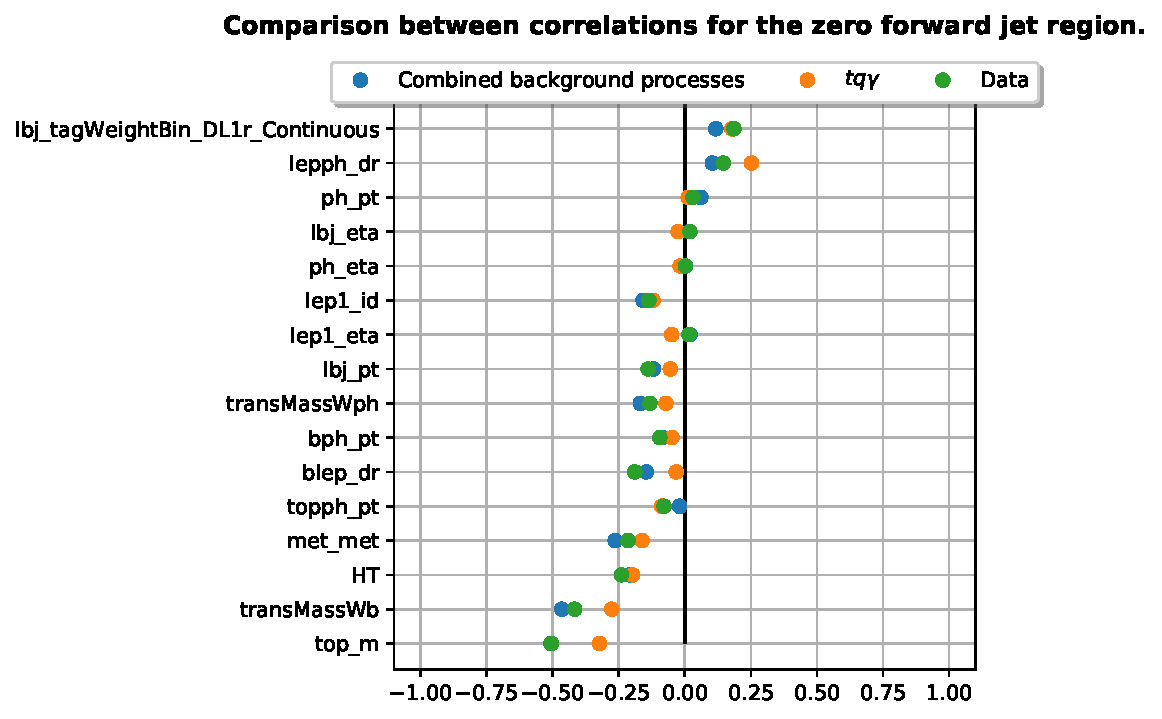
\includegraphics[width=0.7\textwidth]{Plots/corr0fjvariables.pdf}
    \caption{Visualisation of the correlations of input variables with the NN output in the $0\,fj$ region for the background samples, $tq\gamma$ and the measured data.}
    \label{fig:corr0fj}
\end{figure}
\begin{figure}
    \centering
    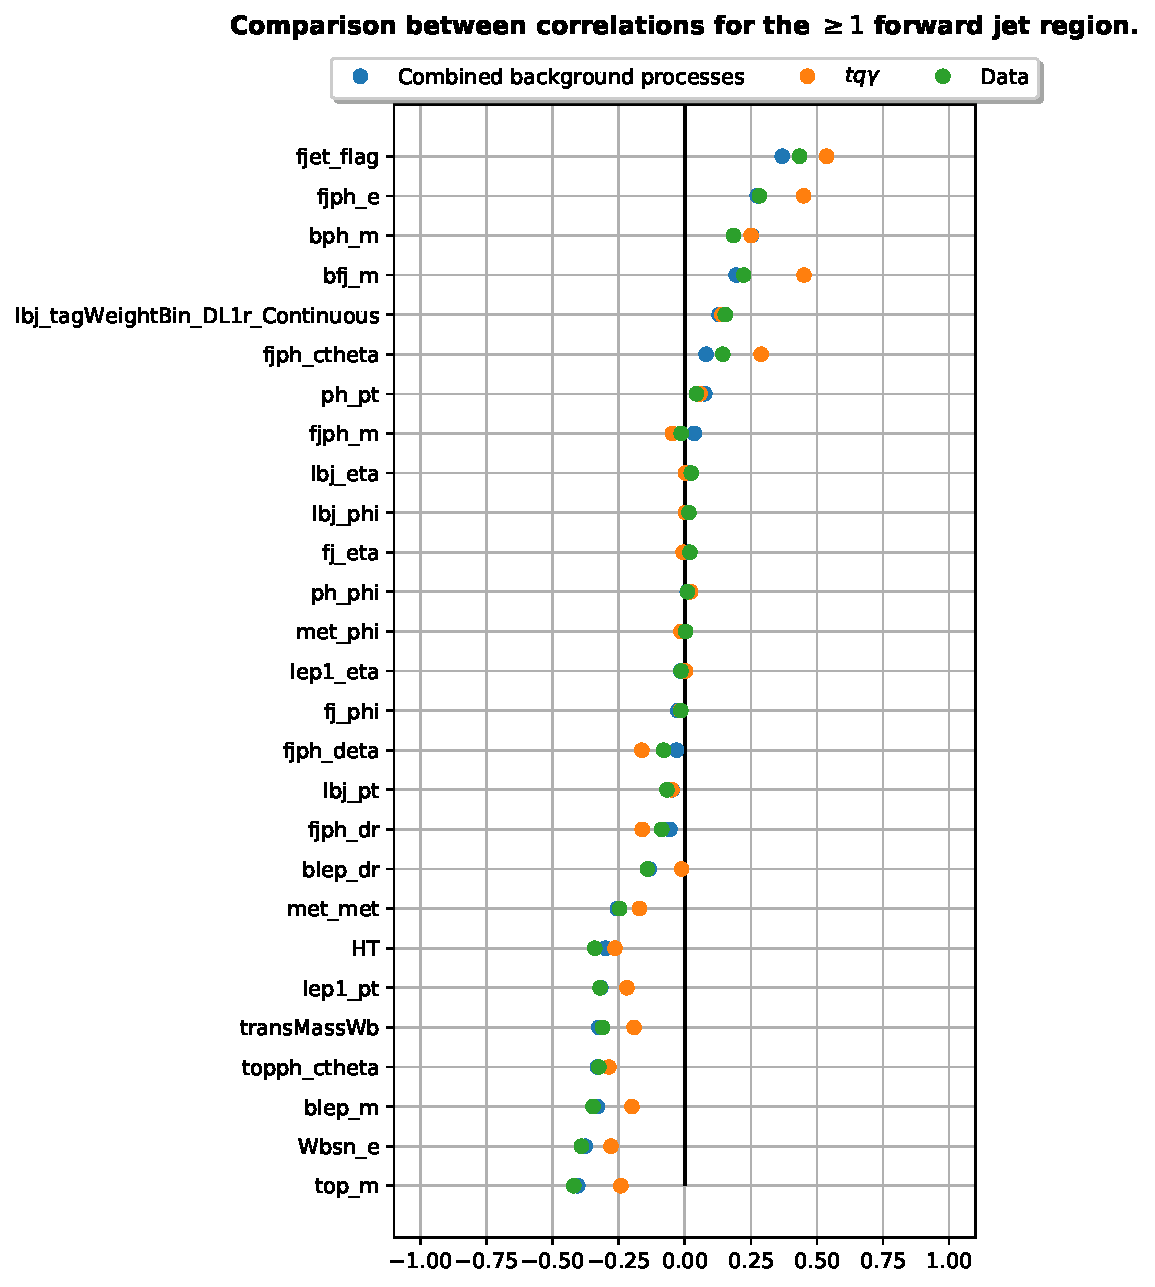
\includegraphics[width=0.7\textwidth]{Plots/corr1fjvariables1.pdf}
    \caption{Visualisation of the correlations of input variables with the NN output in the $\geq 1\,fj$ region for the background samples, $tq\gamma$ and the measured data.}
    \label{fig:corr1fj}
\end{figure} 

\section{NN output distribution dependence on photon \texorpdfstring{$p_T^\gamma$}{pTGamma} and fjet+photon energy \texorpdfstring{$E_{fj\text{+}\gamma}$}{}}
\label{sec:dependence}

In this section, two input variables are chosen to analyse the influence on the NN output further. In the first part of the analysis, an energy region for the input variables is chosen. Then, only events within that energy region are considered. This will be referred to as a "cut" throughout this section. 
After the cut, the distribution of the NN output is plotted to determine any noticeable changes. Additionally, a threshold for the NN output is chosen, and every event above the threshold is considered as a signal. The signal above the threshold must not exceed a statistical error $\frac{N_\text{signal}}{\sqrt{N_\text{signal}}}$ of over $10\%$. 
The composition of events above the threshold is then visualised and discussed. Changes in signal and background compositions are examined. For simplicity, only the $\geq 1$ forward jet region is considered in this analysis.

To compare with the NN output before any cut is applied, the Figure~\ref{fig:full} gives the composition of NN output for two different threshholds. One at $NN = 0.9$ and the other at the highest possible threshhold before the statistical error becomes too high.
\begin{figure}
    \centering
    \begin{subfigure}[b]{0.6\textwidth}
       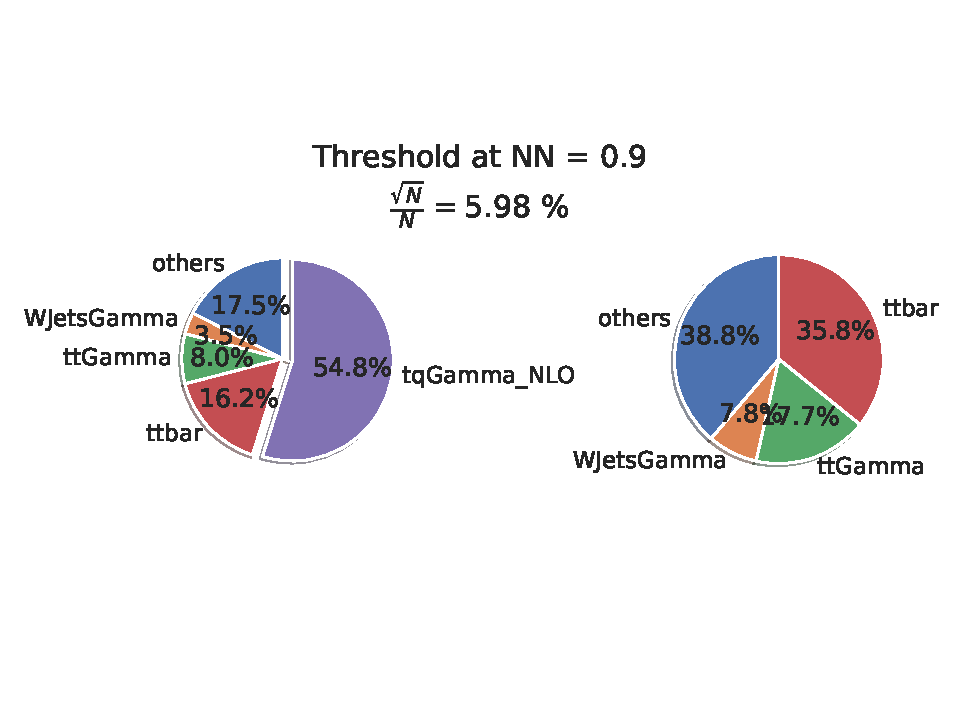
\includegraphics[width=1\linewidth]{Plots/composition9FULL.pdf}
    \end{subfigure}
    
    \begin{subfigure}[b]{0.6\textwidth}
       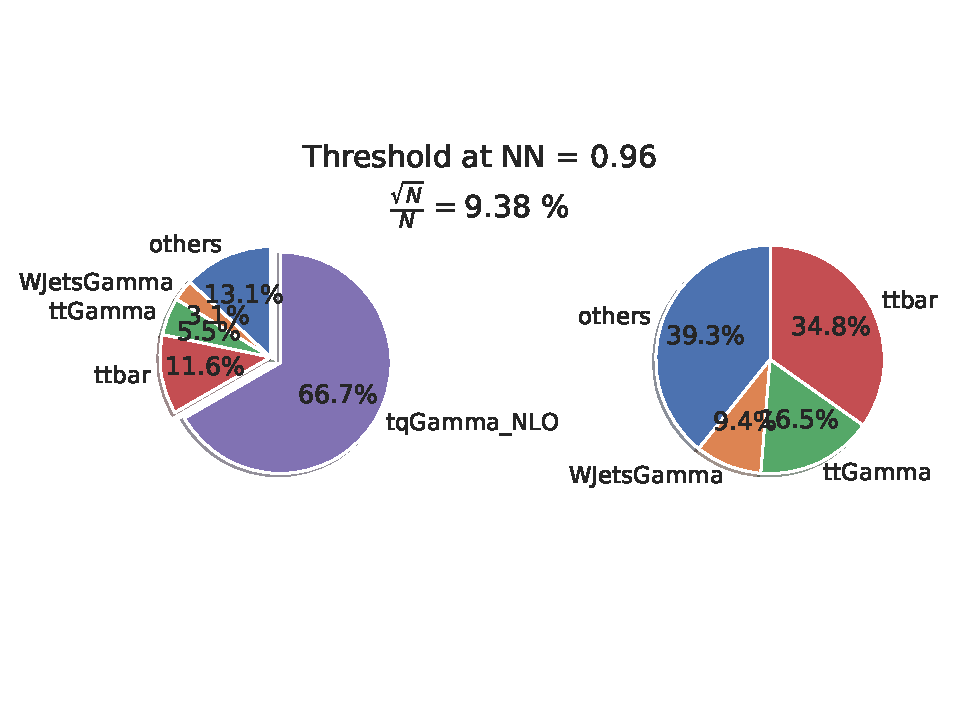
\includegraphics[width=1\linewidth]{Plots/compositionTenFULL.pdf}
    \end{subfigure}
    \caption{Composition of NN output for two different threshholds without any cuts applied. The right pie chart gives the composition without of the background.}
    \label{fig:full}
\end{figure}

The first input variable that is to be analysed is the transverse momentum of the photon $p_T^\gamma$. As the $tq\gamma$ process is sensitive to the top quark to photon coupling, analysing the output dependence of the momentum of the photon provides a good way to test this prediction. 
Results from \autoref{sec:corrvis} give a low correlation of $p_T^\gamma$ at around $15.5\%$ in the $\geq 1\, fj$ region. The dependence of the NN output on $p_T^\gamma$ is therefore found not to be significant. The composition still remains of interest. 

The distribution of $p_T^\gamma$ is shown in \autoref{fig:ph_pt}. 

\begin{figure}[htbp]
    \centering
    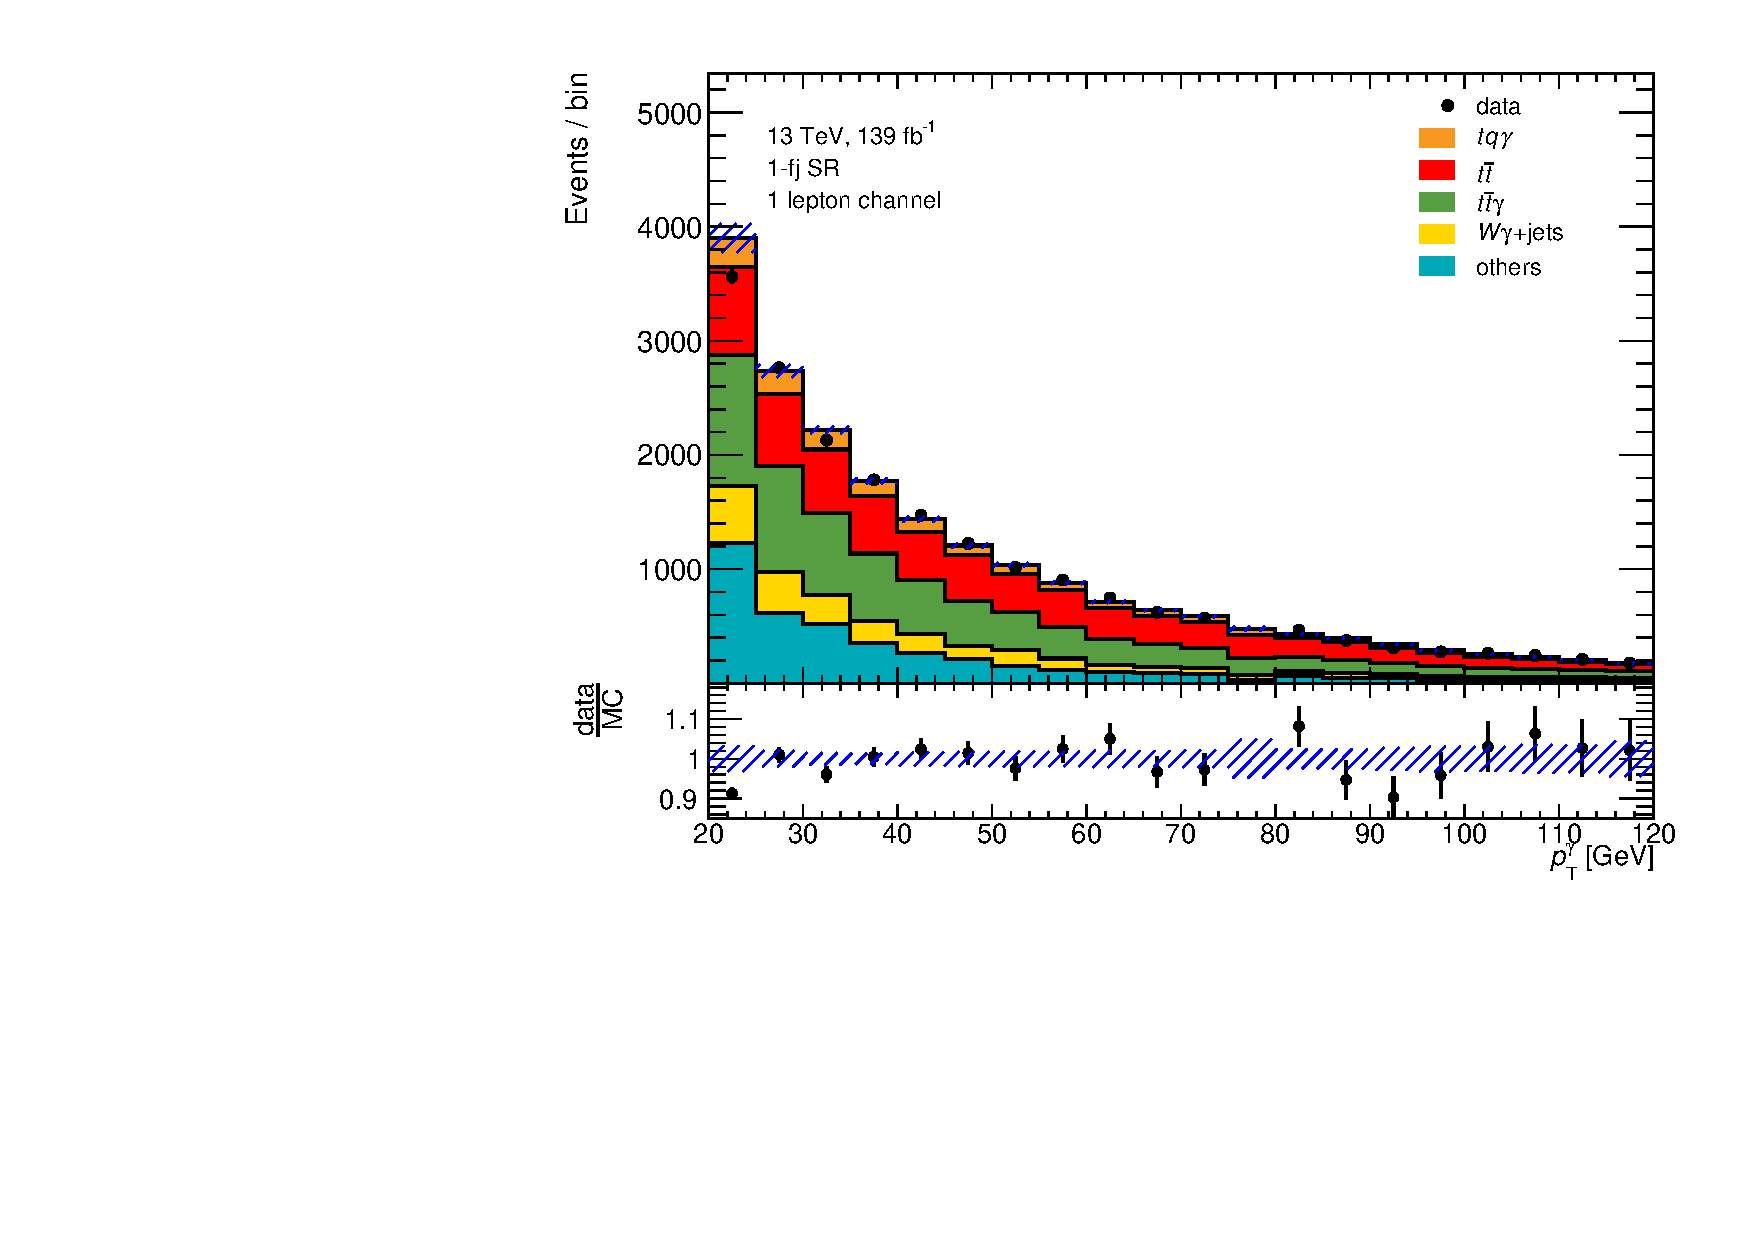
\includegraphics[width=0.6\textwidth]{Plots/ph_pt.pdf}
    \caption{Distribution of the transverse momentum of the photon $p_T^\gamma$.}
    \label{fig:ph_pt}
\end{figure}

With the help of the distribution it is chosen to cut $p_T^\gamma$ at $40\,\si{\giga\electronvolt}$. The positive correlation predicts that higher $p_T^\gamma$ result in a better signal-background discrimination in the NN output. 
The NN output distribution for events with $p_T^\gamma \geq 40\,\si{\giga\electronvolt}$ is displayed in \autoref{fig:outputA40ph}. The composition after two different threshholds is shown in \autoref{fig:phptA40}.

\begin{figure}
    \centering
    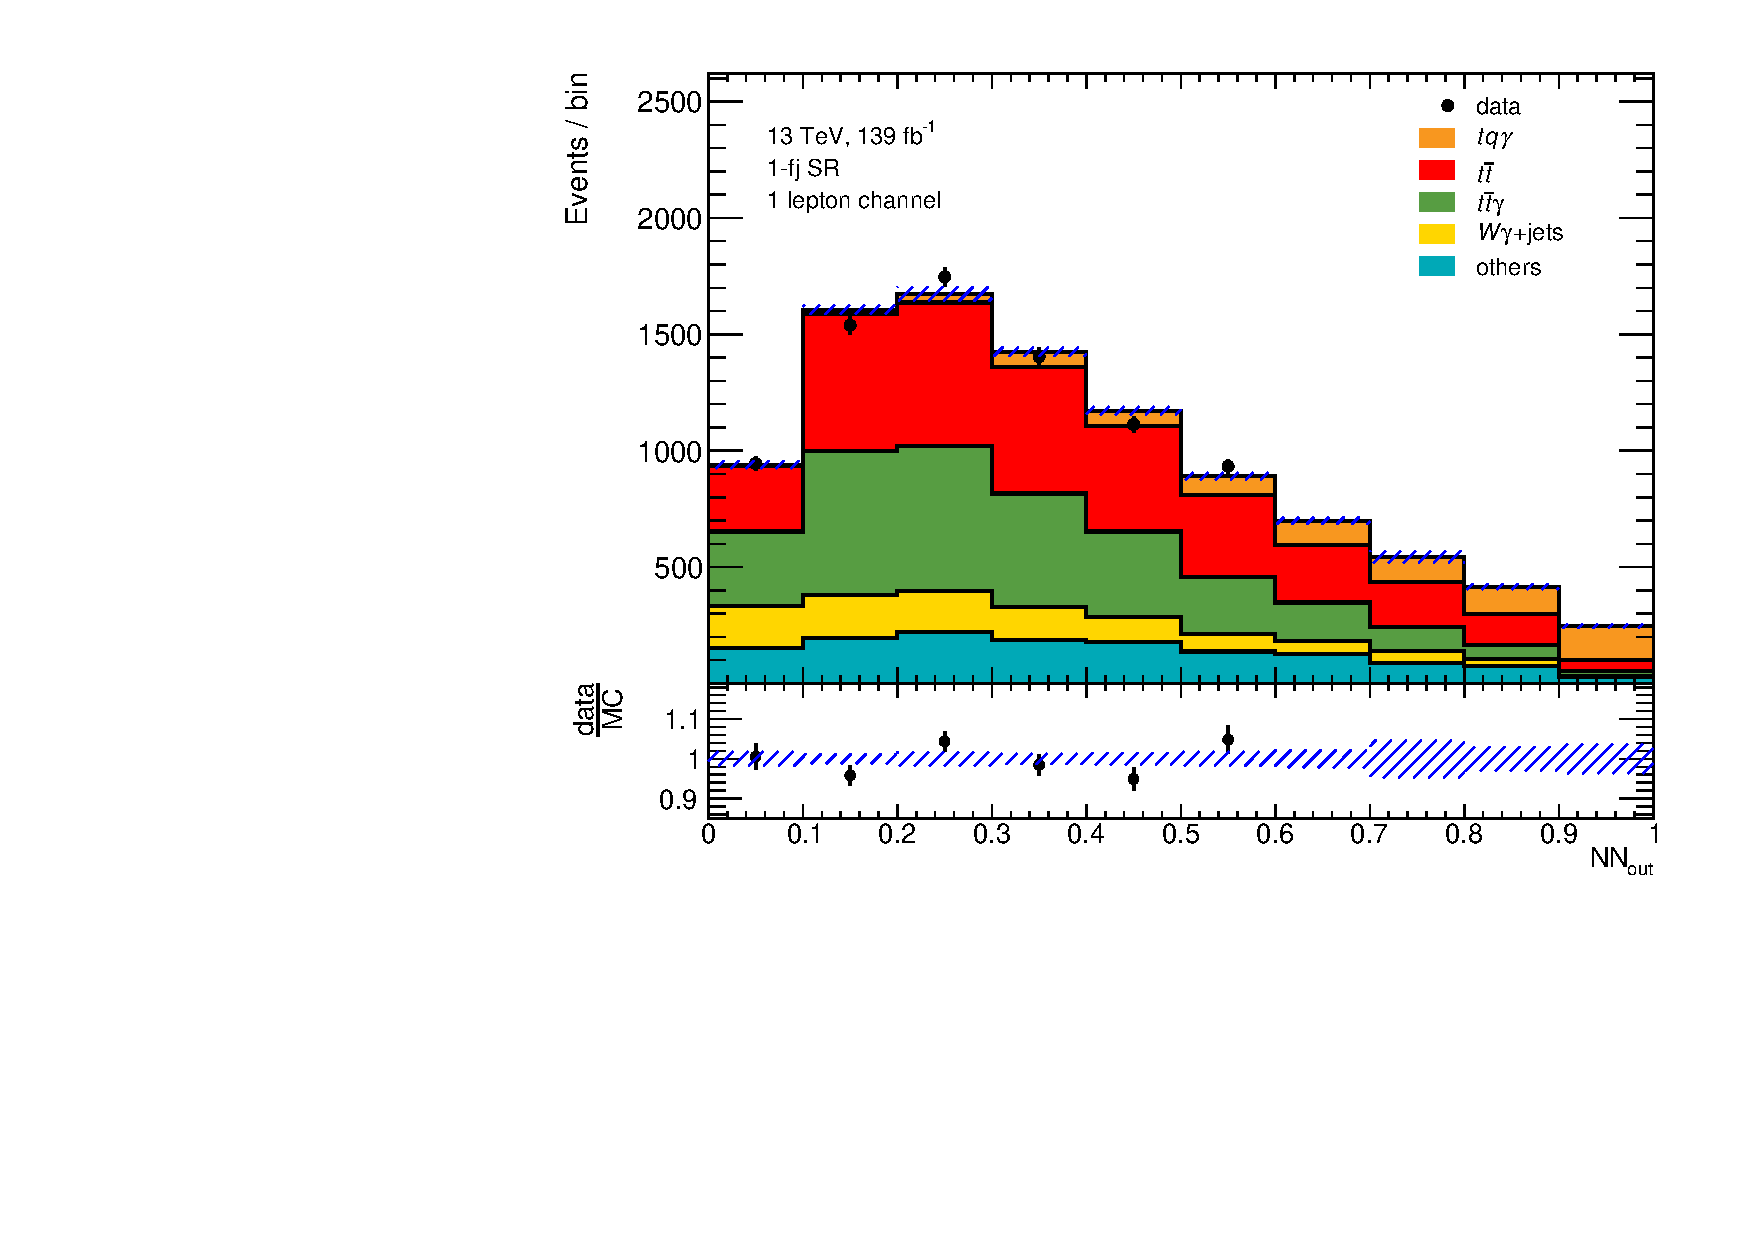
\includegraphics[width=0.7\textwidth]{Plots/NN_out_mixphA40.pdf}
    \caption{NN output distribution for the $p_T^\gamma \geq 40\,\si{\giga\electronvolt}$ region.}
    \label{fig:outputA40ph}
\end{figure} 

\begin{figure}
    \centering
    \begin{subfigure}[b]{0.6\textwidth}
       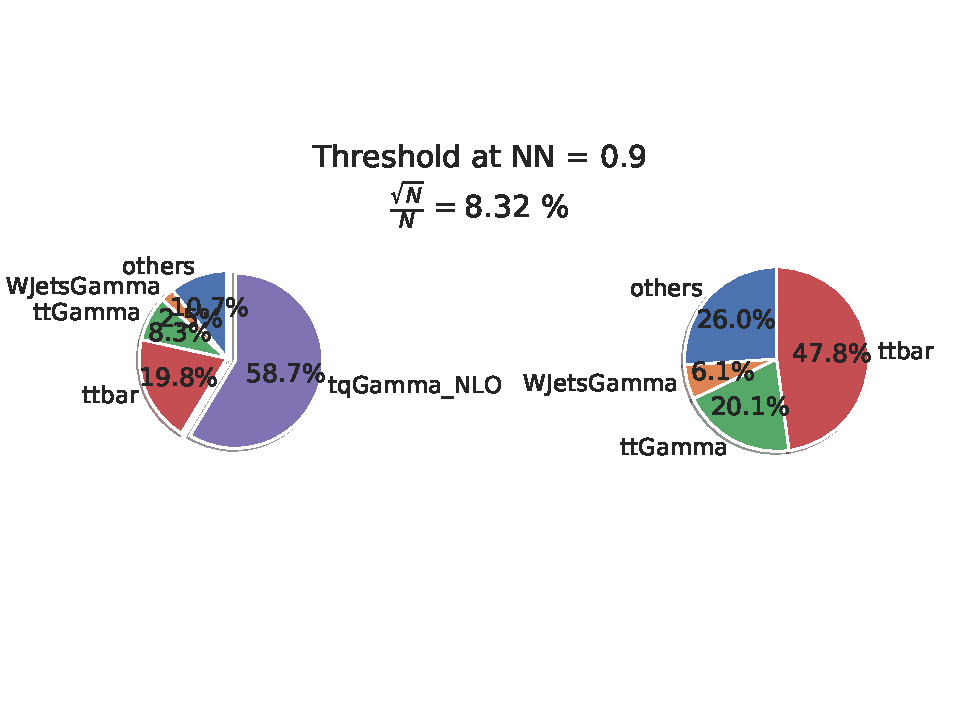
\includegraphics[width=1\linewidth]{Plots/composition9phA40.pdf}
    \end{subfigure}
    
    \begin{subfigure}[b]{0.6\textwidth}
       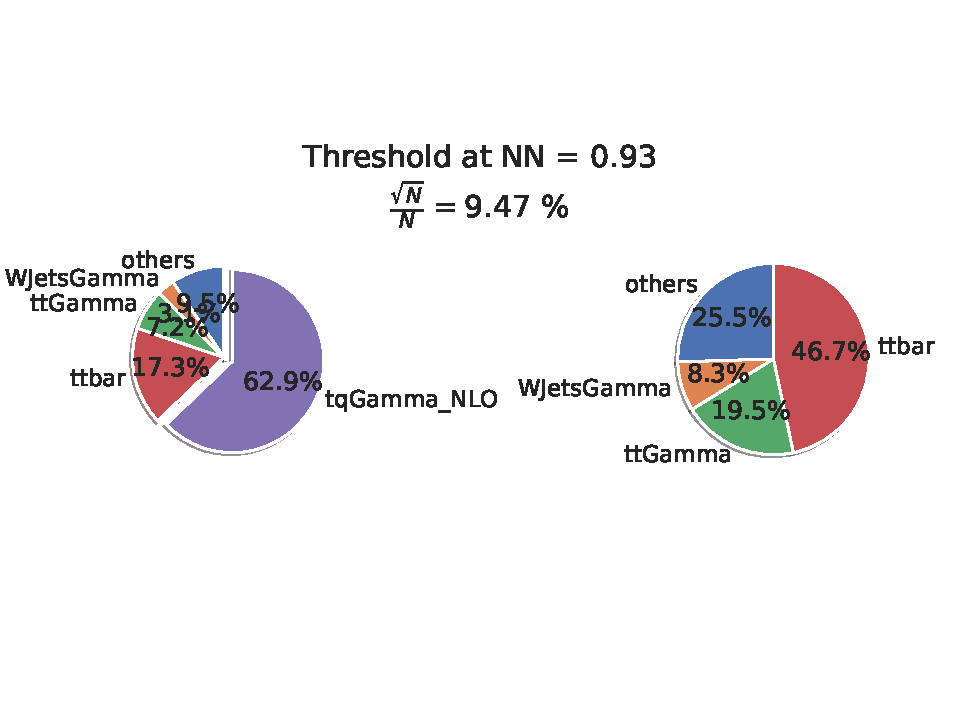
\includegraphics[width=1\linewidth]{Plots/compositionTenphA40.pdf}
    \end{subfigure}
    \caption{Composition of NN output for two different threshholds in the region $p_T^\gamma \geq 40\,\si{\giga\electronvolt}$. }
    \label{fig:phptA40}
\end{figure}

The distribution of $E_{fj\text{+}\gamma}$ is shown in \autoref{fig:fjph_e}. $E_{fj\text{+}\gamma}$ is chosen to be cut to the region $E_{fj\text{+}\gamma} \geq 900\,\si{\giga\electronvolt}$. 
Significant correlation 

\begin{figure}
    \centering
    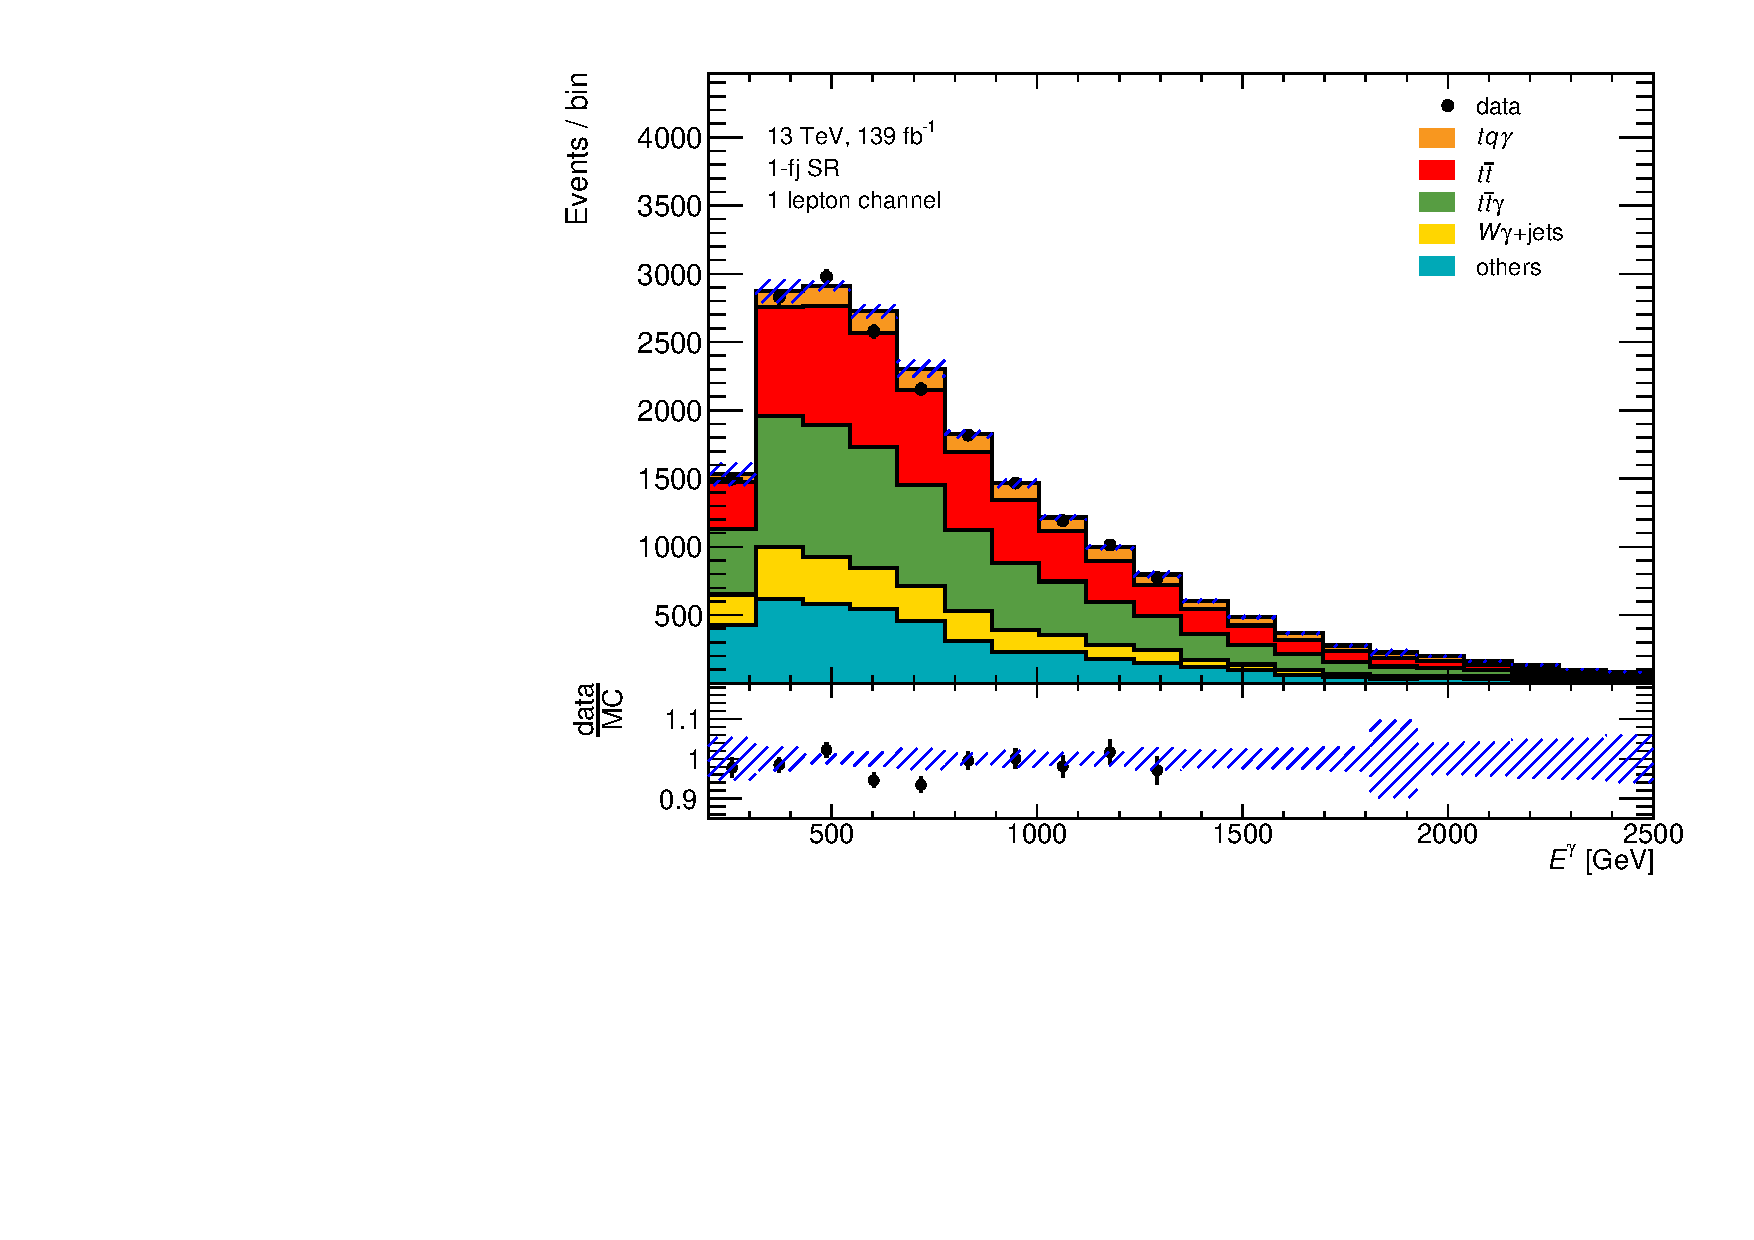
\includegraphics[width=0.7\textwidth]{Plots/fjph_e.pdf}
    \caption{Distribution of the forward jet + photon energy $E_{fj\text{+}\gamma}$.}
    \label{fig:fjph_e}
\end{figure} 

\begin{figure}
    \centering
    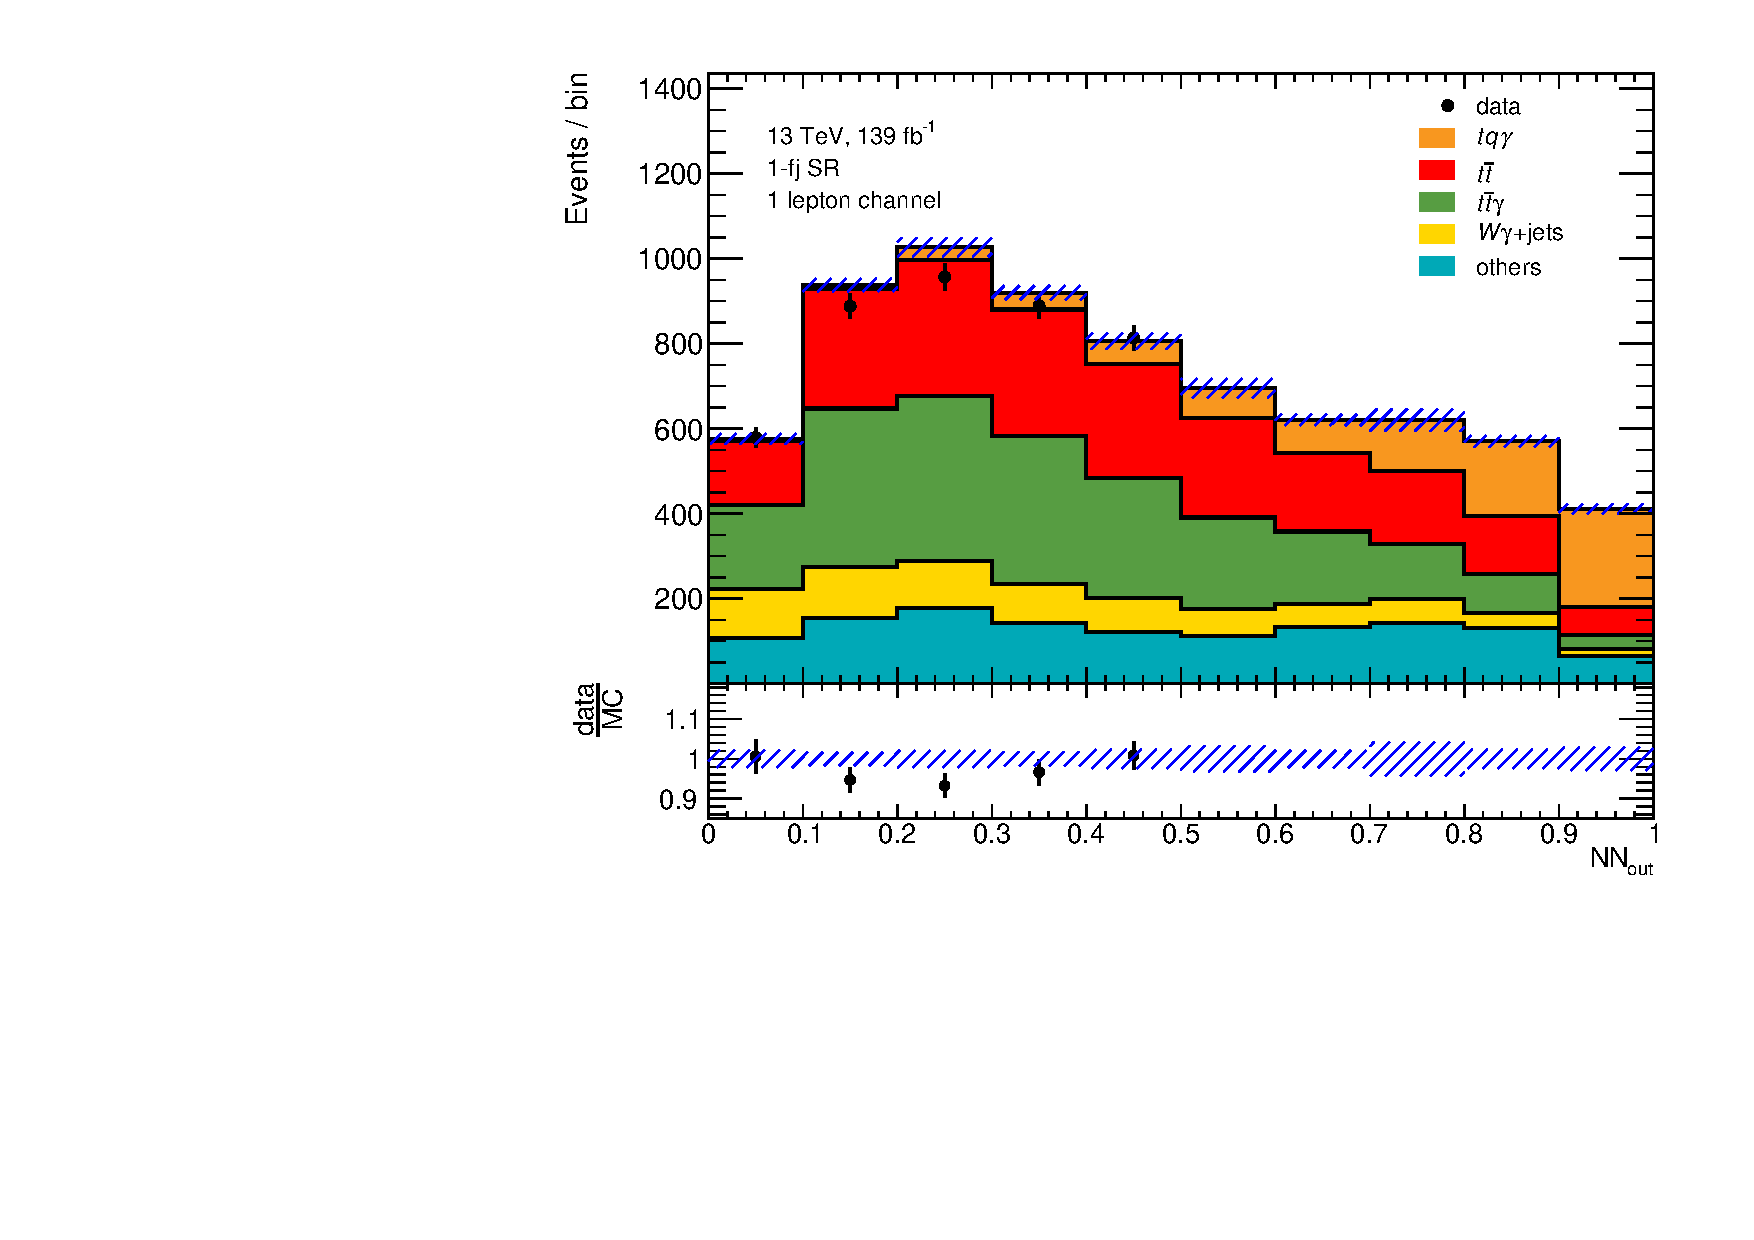
\includegraphics[width=0.7\textwidth]{Plots/NN_out_mixfjphA900.pdf}
    \caption{NN output distribution for the $E_{fj\text{+}\gamma} \geq 900\,\si{\giga\electronvolt}$ region.}
    \label{fig:outputA900fjph_e}
\end{figure} 

\begin{figure}
    \centering
    \begin{subfigure}[b]{0.6\textwidth}
       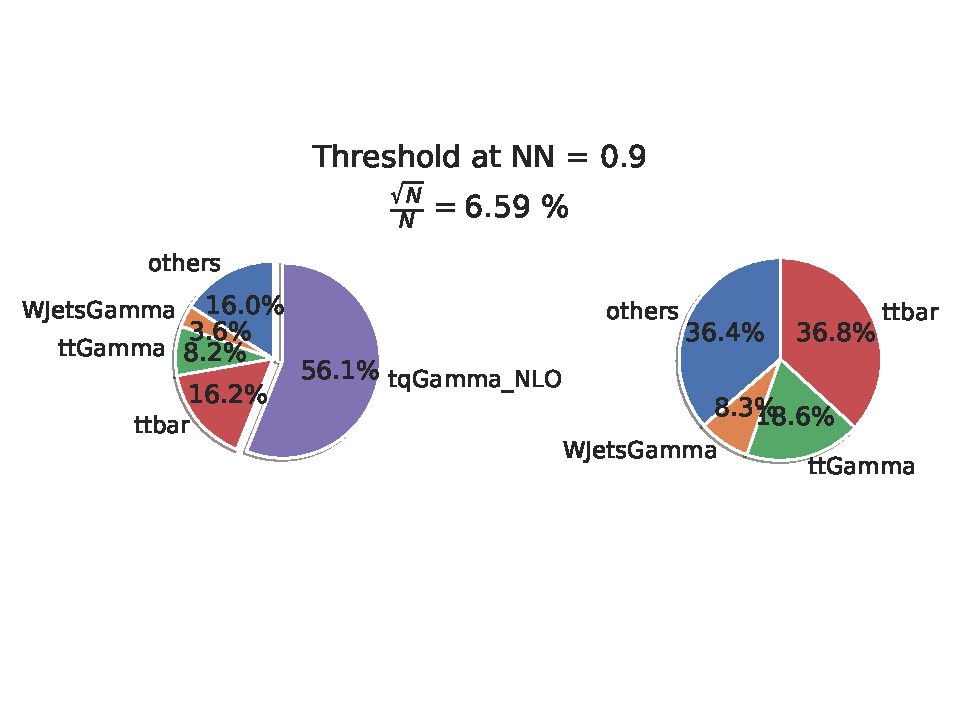
\includegraphics[width=1\linewidth]{Plots/composition9fjA900.pdf}
    \end{subfigure}
    
    \begin{subfigure}[b]{0.6\textwidth}
       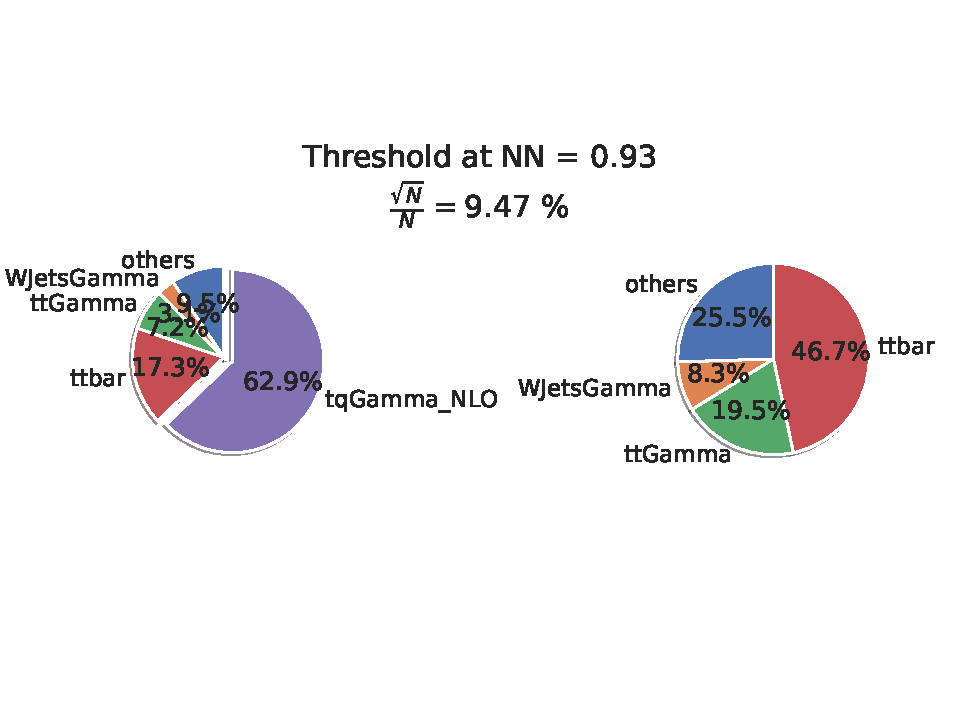
\includegraphics[width=1\linewidth]{Plots/compositionTenphA40.pdf}
    \end{subfigure}
    \caption{Composition of NN output for two different threshholds in the region $E_{fj\text{+}\gamma} \geq 900\,\si{\giga\electronvolt}$. }
    \label{fig:fjph_eA900comp}
\end{figure}
\chapter{Conclusion}
The influence of different input variables on the NN output has been thoroughly analyzed. It has been calculated how the characteristic features of the $tq\gamma$ process 
correlate with the output. Highly correlated and less correlated features are identified, and the reasons for high or low correlation are discussed. 
Most correlations follow the expectations, verifying the correctness of the calculations.

Two input features, the transverse momentum of the photon $p_T^\gamma$ and the sum of the forward jet energies and the photon energy $E_{fj\text{+}\gamma}$, have been further examined. 
For $p_T^\gamma$, it has been found that higher divisions in energy, such as the division into the region $p_T^\gamma > 40 \,\si{\giga\electronvolt}$, result in more efficient signal-background separations (higher values for $\frac{S}{\sqrt{B}}$) in the NN output than lower energy divisions. 
While this observation is significant, it is not as substantial as the effects of divisions for the $E_{fj\text{+}\gamma}$ input feature. The much higher correlation of $E_{fj\text{+}\gamma}$ leads to more significant changes in the NN output for different divisions. 
For this feauture, it is again found that higher energies, such as the region $E_{fj\text{+}\gamma} > 1 \,\si{\tera\electronvolt}$, ensues substantially better seperation in the NN output. 

All in all, the goal of this thesis has been achieved successfully. This thesis provides an essential framework for the differential measurement of $tq\gamma$ with the full Run-2 dataset of the LHC. It provides an overview of different input variables concerning the influence on the NN output. 
Furthermore, it is shown that divisions on different input features are well suited for optimising of signal-background discrimination in the NN output. Additionally, it is also confirmed that the significance of divisions on input features coincide with the calculated correlations. 
The framework provided by this thesis may be used to inspect different input variables further. Due to the scope of the thesis, additional inspections of the input features with regard to the NN were not made.
\chapter{Appendix}
\begin{table}[htbp]
    \centering
    \begin{tabular}{c|c c c|c c c}
        \toprule
        {}&\multicolumn{3}{c}{$0\, fj$ region}&\multicolumn{3}{c}{$\geq 1\, fj$ region}\\
        Event parameter &  Background &  $tq\gamma$ &  Data &  Background &  $tq\gamma$ &  Data \\
        \midrule
        top\_m                            & -0.51 &      0.01 &   0.03 & -0.41 &      0.06 &   0.04 \\ \hline
        Wbsn\_e                           & -0.35 &     -0.02 &   0.00 & -0.38 &      0.00 &  -0.00 \\ \hline
        blep\_m                           & -0.39 &      0.01 &   0.01 & -0.33 &      0.02 &   0.01 \\ \hline
        topph\_ctheta                     & -0.28 &     -0.00 &     & -0.33 &     -0.01 &   0.02 \\ \hline
        transMassWb                      & -0.47 &     -0.00 &     & -0.33 &     -0.02 &  -0.02 \\ \hline
        lep1\_pt                          & -0.36 &        &     & -0.32 &      0.54 &   0.43 \\ \hline
        HT                               & -0.21 &     -0.24 &  -0.35 & -0.30 &     -0.22 &  -0.32 \\ \hline
        met\_met                          & -0.26 &     -0.05 &   0.02 & -0.26 &      0.00 &  -0.01 \\ \hline
        topph\_pt                         & -0.02 &     -0.12 &  -0.14 & -0.18 &     -0.06 &  -0.03 \\ \hline
        blep\_dr                          & -0.15 &     -0.06 &  -0.14 & -0.14 &     -0.05 &  -0.07 \\ \hline
        bph\_pt                           & -0.08 &     -0.03 &   0.02 & -0.13 &      0.00 &   0.02 \\ \hline
        transMassWph                     & -0.17 &      0.00 &  -0.00 & -0.10 &      0.00 &   0.02 \\ \hline
        fjph\_dr                          &  0.00 &      0.18 &   0.19 & -0.06 &      0.14 &   0.15 \\ \hline
        lbj\_pt                           & -0.12 &     -0.32 &  -0.50 & -0.05 &     -0.24 &  -0.42 \\ \hline
        fjph\_deta                        &  0.00 &     -0.36 &  -0.29 & -0.03 &     -0.29 &  -0.33 \\ \hline
        fj\_phi                           & -0.00 &     -0.09 &  -0.08 & -0.03 &     -0.11 &  -0.19 \\ \hline
        lep1\_eta                         &  0.02 &     -0.30 &  -0.37 & -0.02 &     -0.28 &  -0.39 \\ \hline
        met\_phi                          &  0.00 &      0.27 &   0.14 & -0.01 &      0.25 &   0.18 \\ \hline
        lep1\_id                          & -0.16 &     -0.27 &  -0.43 & -0.00 &     -0.20 &  -0.35 \\ \hline
        ph\_eta                           &  0.00 &        &     &  0.00 &      0.45 &   0.22 \\ \hline
        ph\_phi                           & -0.00 &     -0.05 &  -0.09 &  0.01 &     -0.08 &  -0.13 \\ \hline
        fj\_eta                           & -0.00 &        &     &  0.01 &     -0.05 &  -0.01 \\ \hline
        lbj\_phi                          & -0.00 &      0.07 &   0.03 &  0.01 &      0.45 &   0.28 \\ \hline
        lbj\_eta                          &  0.02 &     -0.02 &   0.00 &  0.02 &     -0.16 &  -0.09 \\ \hline
        fjph\_m                           &    &     -0.02 &   0.00 &  0.04 &     -0.16 &  -0.08 \\ \hline
        ph\_pt                            &  0.06 &        &     &  0.08 &      0.29 &   0.14 \\ \hline
        fjph\_ctheta                      &    &      0.25 &   0.15 &  0.08 &      0.12 &   0.12 \\ \hline
        lepph\_dr                         &  0.10 &     -0.03 &  -0.19 &  0.11 &     -0.01 &  -0.14 \\ \hline
        lbj\_tagWeightBin &  0.12 &     -0.16 &  -0.21 &  0.13 &     -0.17 &  -0.25 \\ 
        \_DL1r\_Continuous &&&&&&\\ \hline
        bfj\_m                            &    &      0.02 &  -0.00 &  0.19 &     -0.01 &   0.00 \\ \hline
        bph\_m                            &  0.19 &     -0.20 &  -0.24 &  0.25 &     -0.26 &  -0.34 \\ \hline
        fjph\_e                           &  0.04 &     -0.07 &  -0.13 &  0.27 &     -0.03 &  -0.10 \\ \hline
        fjet\_flag                        &    &     -0.28 &  -0.42 &  0.37 &     -0.19 &  -0.31 \\ \hline
        \bottomrule
        \end{tabular}
    \caption{List of correlations between samples and the NN output in the zero forward jet region as well as samples in the $\geq 1$ forward jet region.}
    \label{tab:corrAll}
\end{table}
\begin{figure}[htbp]
    \centering
    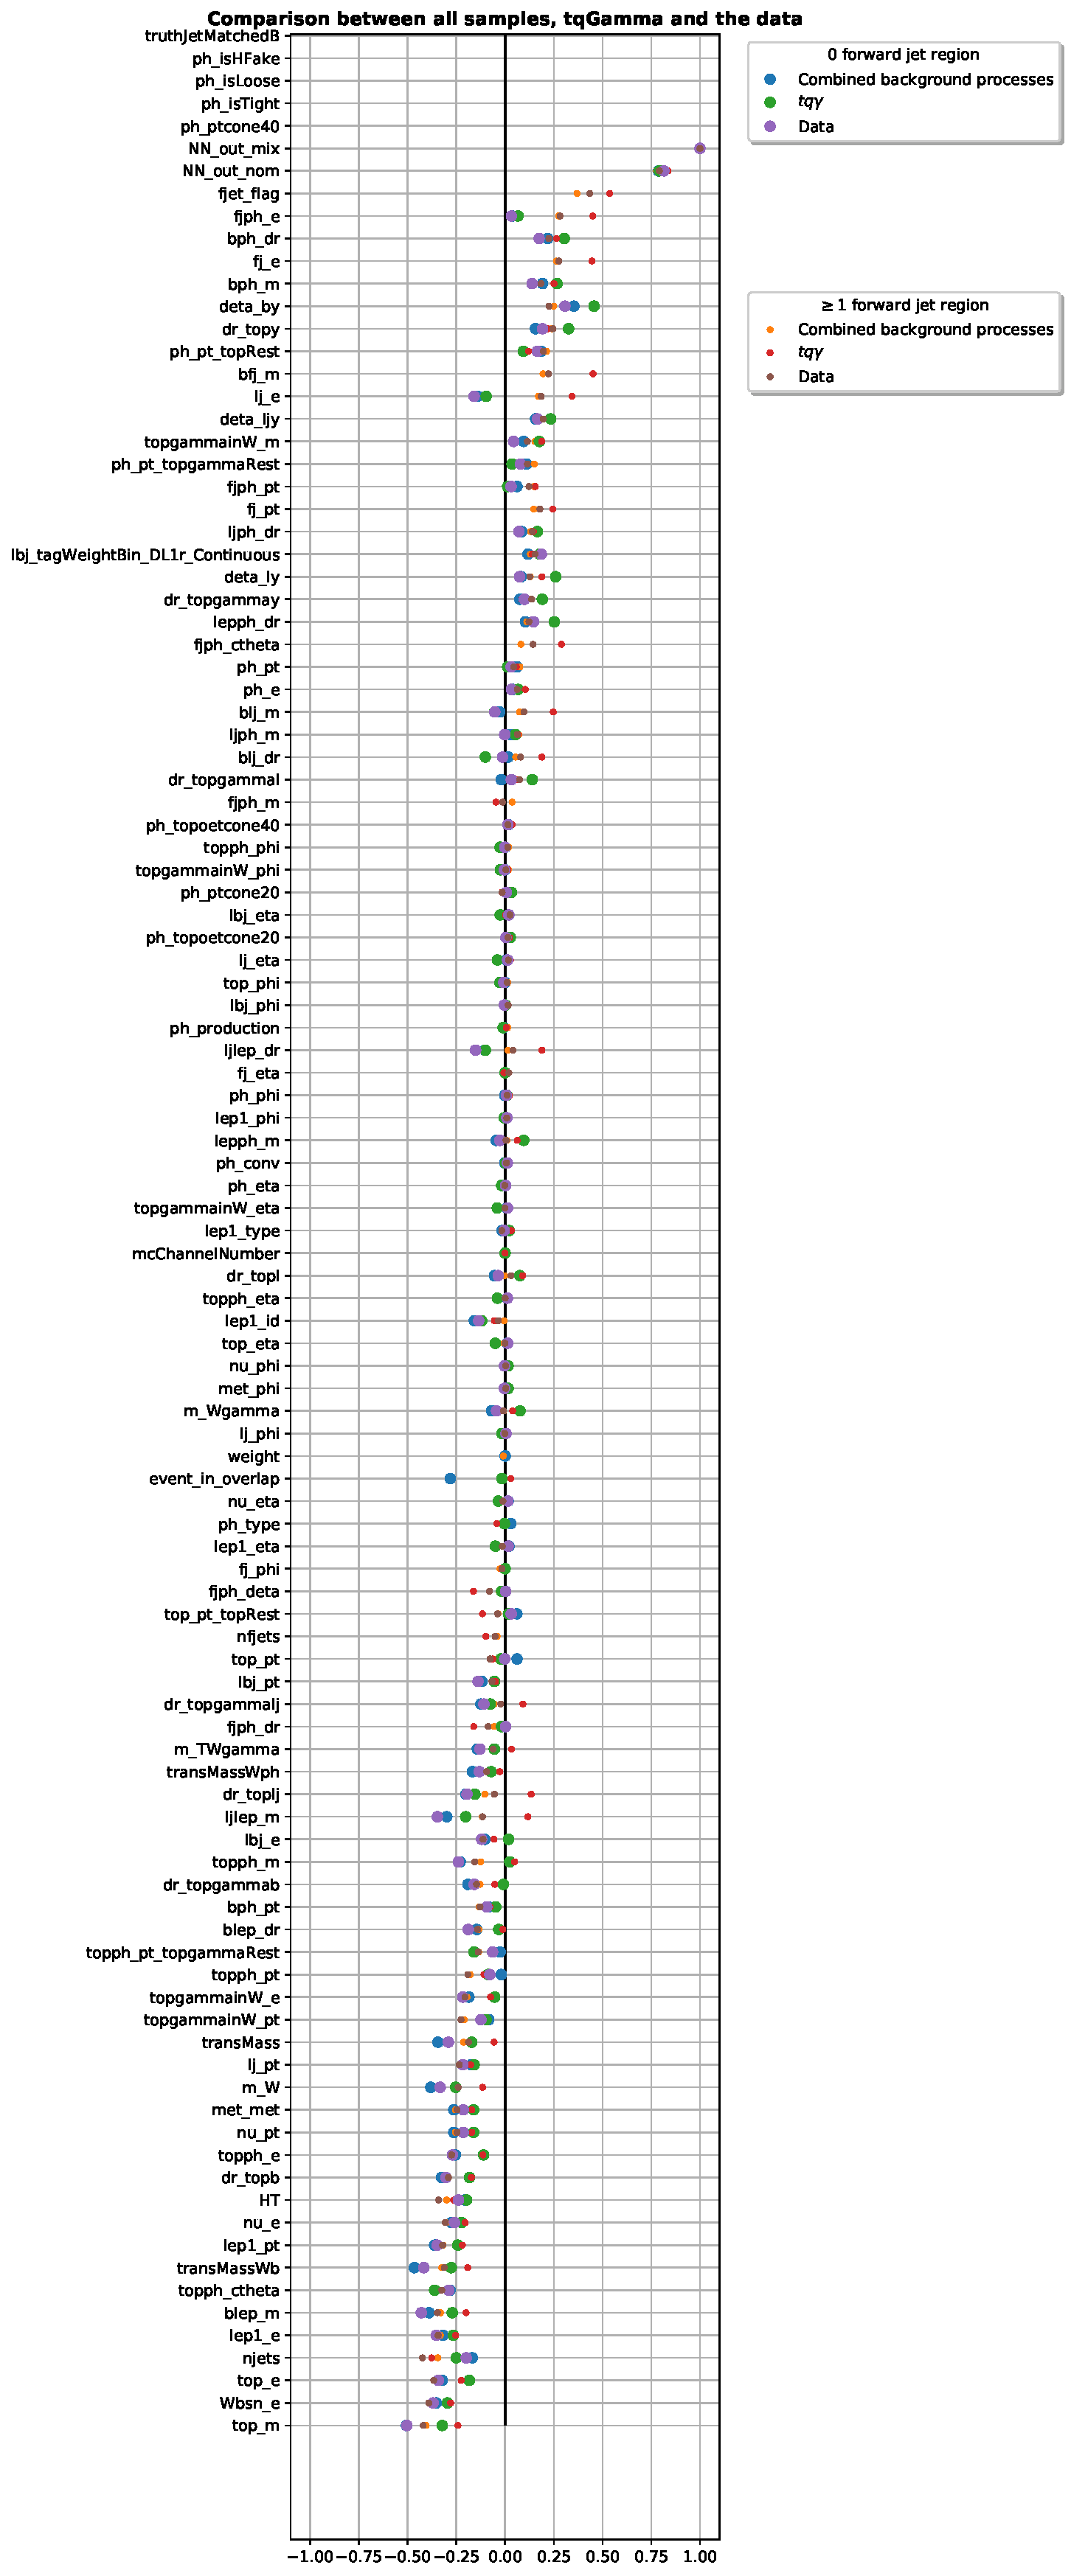
\includegraphics[width=0.7\textwidth]{Plots/corrAll.pdf}
    \caption{Correlations of all event properties with the NN output in the $0\,fj$ and $\geq 1\,fj$ region for the background samples, $tq\gamma$ and the measured data.}
    \label{fig:corrAll}
\end{figure}
\chapter{Danksagung}

Zu aller erst möchte ich mich bei Herrn Priv.-Doz. Dr. Johannes Erdmann bedanken, der mir überhaupt ermöglicht hat, diese Bachelorarbeit in dem Lehrstuhl für Experimentelle Physik IV zu schreiben, 
mich Monate vorher über potentielle Aufgaben und dem Ablauf der Arbeit unterrichtet und mein Interesse an das Thema stets aufrecht erhalten hat.\\
Ich möchte mich auch bei Björn Wendland und Nils Julius Abicht bedanken, die meinen Fortschritt im Auge behalten haben, um den Abschluss der Arbeit zu garantieren, 
und meine Zwischenergebnisse korrekturgelesen haben. \\
Des Weiteren möchte ich mich bei Herrn Prof. Dr. Johannes Albrecht für die Zweitgutachtung herzlich bedanken. \\
Abschließend, bedanke ich mich bei meinen Freunden, die mir stetig in stressigen Momenten Unterstützung gegeben haben, ohne die diese Bachelroarbeit nicht gelungen wäre.  


\appendix
% Hier beginnt der Anhang, nummeriert in lateinischen Buchstaben
\chapter{Ein Anhangskapitel}

Hier könnte ein Anhang stehen, falls Sie z.\,B.\ Code, Konstruktionszeichnungen oder Ähnliches mit in die Arbeit bringen wollen.
Im Normalfall stehen jedoch alle Ihre Resultate im Hauptteil der Bachelorarbeit und ein Anhang ist überflüssig.


\backmatter
\printbibliography

\cleardoublepage
\thispagestyle{empty}
\section*{Eidesstattliche Versicherung}
Ich versichere hiermit an Eides statt, dass ich die vorliegende Abschlussarbeit mit dem Titel \enquote{\thetitle} selbstständig und ohne unzulässige fremde Hilfe erbracht habe.
Ich habe keine anderen als die angegebenen Quellen und Hilfsmittel benutzt, sowie wörtliche und sinngemäße Zitate kenntlich gemacht. 
Die Arbeit hat in gleicher oder ähnlicher Form noch keiner Prüfungsbehörde vorgelegen.

\vspace*{1cm}\noindent
\begin{center}
  \begin{tabular}{@{}p{0.4\textwidth}@{\hspace{0.15\textwidth}}p{0.4\textwidth}@{}}
  \rule{\linewidth}{0.25pt}& \rule{\linewidth}{0.25pt}\\
  Ort, Datum & Unterschrift
  \end{tabular}
\end{center}

\subsection*{Belehrung}
Wer vorsätzlich gegen eine die Täuschung über Prüfungsleistungen betreffende Regelung einer Hochschulprüfungsordnung verstößt, handelt ordnungswidrig.
Die Ordnungswidrigkeit kann mit einer Geldbuße von bis zu \SI[round-mode=places, round-precision=2]{50000}{€} geahndet werden. 
Zuständige Verwaltungsbehörde für die Verfolgung und Ahndung von Ordnungswidrigkeiten ist der Kanzler/die Kanzlerin der Technischen Universität Dortmund. 
Im Falle eines mehrfachen oder sonstigen schwerwiegenden Täuschungsversuches kann der Prüfling zudem exmatrikuliert werden \mbox{(\S\,63 Abs. 5 Hochschulgesetz --HG--).}

Die Abgabe einer falschen Versicherung an Eides statt wird mit Freiheitsstrafe bis zu 3 Jahren oder mit Geldstrafe bestraft.

Die Technische Universität Dortmund wird ggf.\ elektronische Vergleichswerkzeuge (wie z.\,B.\ die Software \enquote{turnitin}) zur Überprüfung von Ordnungswidrigkeiten in Prüfungsverfahren nutzen. \\[\baselineskip]

\noindent Die oben stehende Belehrung habe ich zur Kenntnis genommen.\\[1cm]
\begin{center}
\begin{tabular}{@{}p{0.4\textwidth}@{\hspace{0.15\textwidth}}p{0.4\textwidth}@{}}
\rule{\linewidth}{0.25pt}& \rule{\linewidth}{0.25pt}\\
Ort, Datum & Unterschrift
\end{tabular}
\end{center}

\end{document}
